\documentclass[main.tex]{subfiles}                                              
\begin{document}

\section{隐式和参数形式}

在几何建模中，表示曲线和曲面的两种最常见的方法是隐式方程和参数函数。

位于 \({xy}\) 平面的曲线的隐式方程具有形式 \(f\left( {x,y}\right)  = 0\) 。该方程描述了曲线上点的 \(x\) 和 \(y\) 坐标之间的隐式关系。对于给定的曲线，该方程在乘法常数的情况下是唯一的。一个例子是单位半径的圆，其中心位于原点，由方程 \(f\left( {x,y}\right)  = {x}^{2} + {y}^{2} - 1 = 0\) 指定(图 1.1)。

%\begin{center}
%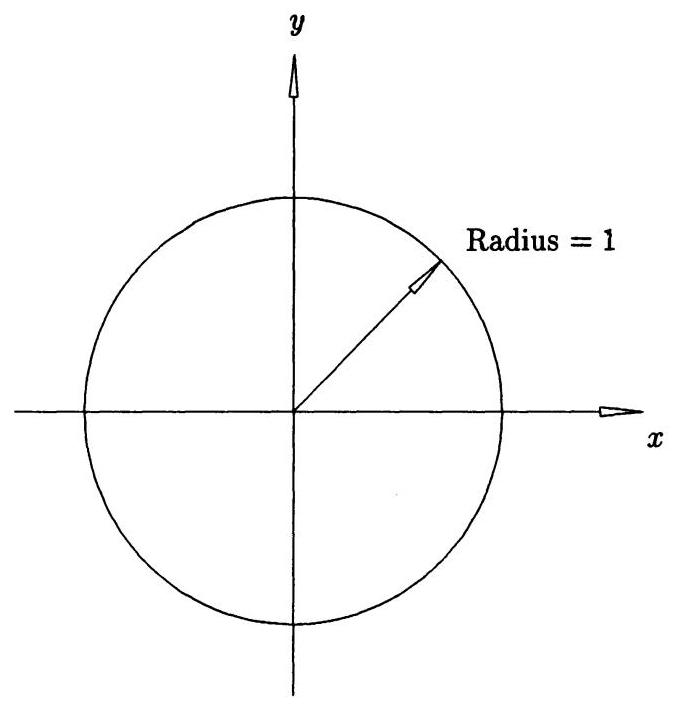
\includegraphics[max width=0.7\textwidth]{images/0193ba0d-ab19-7138-9798-cb281ce60de0_13_435_254_674_704_0.jpg}
%\end{center}
%\hspace*{3em} 

\begin{figure}[ht]
    \centering
    \begin{tikzpicture}
        % 画坐标轴
        \draw[->] (-1.5, 0) -- (1.5, 0) node[right] {$x$};
        \draw[->] (0, -1.5) -- (0, 1.5) node[above] {$y$};

        % 画圆
        \draw[] (0,0) circle(1);

        % 画半径线
        \draw[->] (0,0) -- (0.707, 0.707) node[right];

        % 标记半径长度
        \node at (1.0,1.0) {R = 1};
    \end{tikzpicture}
    \caption{半径为 1，中心位于原点的圆}\label{fig:unit_circle}
\end{figure}

在参数形式中，曲线上点的每个坐标都作为独立参数的显式函数单独表示。

\[
\mathbf{C}\left( u\right)  = \left( {x\left( u\right) ,y\left( u\right) }\right) \;a \leq  u \leq  b
\]

因此， \(\mathbf{C}\left( u\right)\) 是独立变量 \(u\) 的向量值函数。尽管区间 \(\left\lbrack  {a,b}\right\rbrack\) 是任意的，但通常归一化为 \(\left\lbrack  {0,1}\right\rbrack\) 。图 1.1 中所示的圆的第一象限由参数函数定义。

\[
x\left( u\right)  = \cos \left( u\right)
\]

\[
y\left( u\right)  = \sin \left( u\right) \;0 \leq  u \leq  \frac{\pi }{2} \tag{1.1}
\]

设置 \(t = \tan \left( {u/2}\right)\) ，可以推导出替代表示。

\[
x\left( t\right)  = \frac{1 - {t}^{2}}{1 + {t}^{2}}
\]

\[
y\left( t\right)  = \frac{2t}{1 + {t}^{2}}\;0 \leq  t \leq  1 \tag{1.2}
\]

因此，曲线的参数表示并不是唯一的。


将 \(\mathbf{C}\left( u\right)  = \left( {x\left( u\right) ,y\left( u\right) }\right)\) 理解为粒子随时间变化所描绘的路径是很有启发性的； \(u\) 是时间变量， \(\left\lbrack  {a,b}\right\rbrack\) 是时间间隔。 \(\mathbf{C}\left( u\right)\) 的一阶和二阶导数分别是粒子的速度和加速度。对方程 (1.1) 和 (1.2) 进行一次求导得到速度函数。

\[
{\mathbf{C}}^{\prime }\left( u\right)  = \left( {{x}^{\prime }\left( u\right) ,{y}^{\prime }\left( u\right) }\right)  = \left( {-\sin \left( u\right) ,\cos \left( u\right) }\right)
\]

\[
{\mathbf{C}}^{\prime }\left( t\right)  = \left( {{x}^{\prime }\left( t\right) ,{y}^{\prime }\left( t\right) }\right)  = \left( {\frac{-{4t}}{{\left( 1 + {t}^{2}\right) }^{2}},\frac{2\left( {1 - {t}^{2}}\right) }{{\left( 1 + {t}^{2}\right) }^{2}}}\right)
\]

注意，速度向量 \({\mathbf{C}}^{\prime }\left( u\right)\) 的大小是一个常数。

\[
\left| {{\mathbf{C}}^{\prime }\left( u\right) }\right|  = \sqrt{{\sin }^{2}\left( u\right)  + {\cos }^{2}\left( u\right) } = 1
\]

即，粒子的方向随时间变化，但其速度保持不变。这被称为均匀参数化。将 \(t = 0\) 和 \(t = 1\) 代入 \({\mathbf{C}}^{\prime }\left( t\right)\) 得到 \({\mathbf{C}}^{\prime }\left( 0\right)  = \left( {0,2}\right)\) 和 \({\mathbf{C}}^{\prime }\left( 1\right)  = \left( {-1,0}\right)\) ，即，粒子的起始速度是其结束速度的两倍(图 1.2)。

表面由形式为 \(f\left( {x,y,z}\right)  = 0\) 的隐式方程定义。一个例子是以原点为中心的单位半径球体，如图 1.3 所示，并由方程 \({x}^{2} + {y}^{2} + {z}^{2} - 1 = 0\) 指定。同一球体的参数化表示(不唯一)由 \(\mathbf{S}\left( {u,v}\right)  = \left( {x\left( {u,v}\right) ,y\left( {u,v}\right) ,z\left( {u,v}\right) }\right)\) 给出，其中

\[
x\left( {u,v}\right)  = \sin \left( u\right) \cos \left( v\right)
\]

\[
y\left( {u,v}\right)  = \sin \left( u\right) \sin \left( v\right)
\]

\[
z\left( {u,v}\right)  = \cos \left( u\right) \;0 \leq  u \leq  \pi ,0 \leq  v \leq  {2\pi } \tag{1.3}
\]

%\begin{center}
%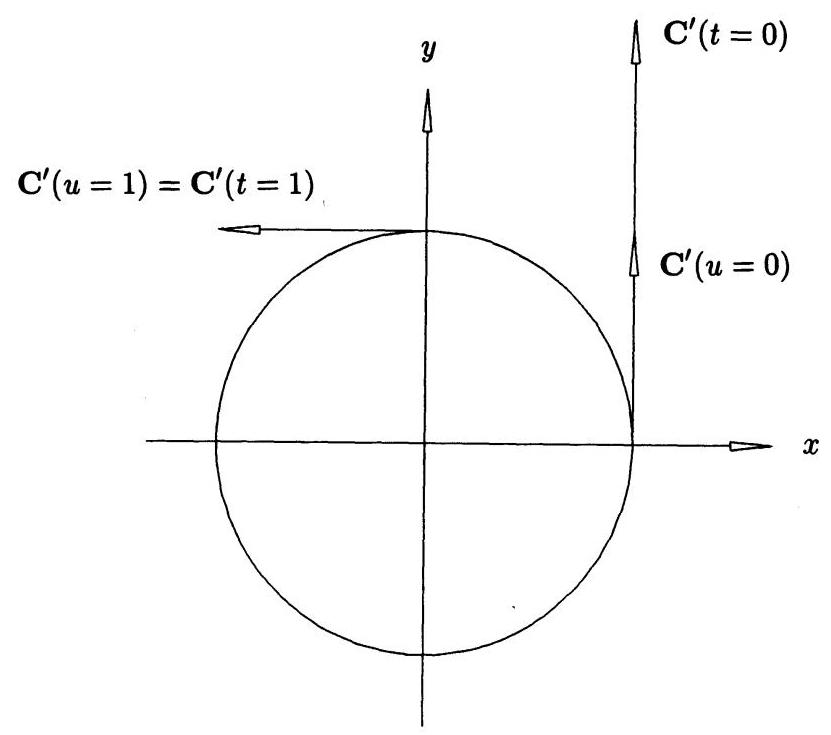
\includegraphics[max width=0.7\textwidth]{images/0193ba0d-ab19-7138-9798-cb281ce60de0_14_357_267_831_735_0.jpg}
%\end{center}
%\hspace*{3em} 

\begin{figure}[ht]
    \centering
    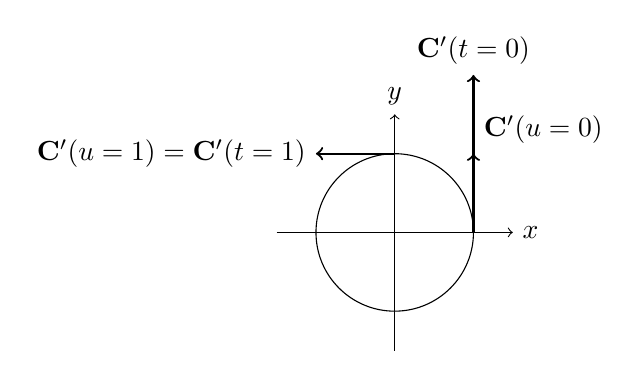
\begin{tikzpicture}
        % 坐标轴
        \draw[->] (-1.5,0) -- (1.5,0) node[right] {$x$};
        \draw[->] (0,-1.5) -- (0,1.5) node[above] {$y$};
        % 圆
        \draw (0,0) circle (1);
        % 导数向量
        \draw[->, thick] (1,0) -- (1,1) node[above right] {$\mathbf{C}'(u=0)$};
        \draw[->, thick] (0,1) -- (-1,1) node[left] {$\mathbf{C}'(u=1)=\mathbf{C}'(t=1)$};
        \draw[->, thick] (1,0) -- (1,2) node[above] {$\mathbf{C}'(t=0)$};
    \end{tikzpicture}
    \caption{在 \(u,t = 0\) 和 1 处的速度向量 \({\mathbf{C}}^{\prime }\left( u\right)\) 和 \({\mathbf{C}}^{\prime }\left( t\right)\) 。}\label{fig:unit_circle}
\end{figure}

请注意，定义一个表面需要两个参数。保持 \(u\) 固定并改变 \(v\) 生成球体的纬线；保持 \(v\) 固定并改变 \(u\) 生成经线。

\begin{center}
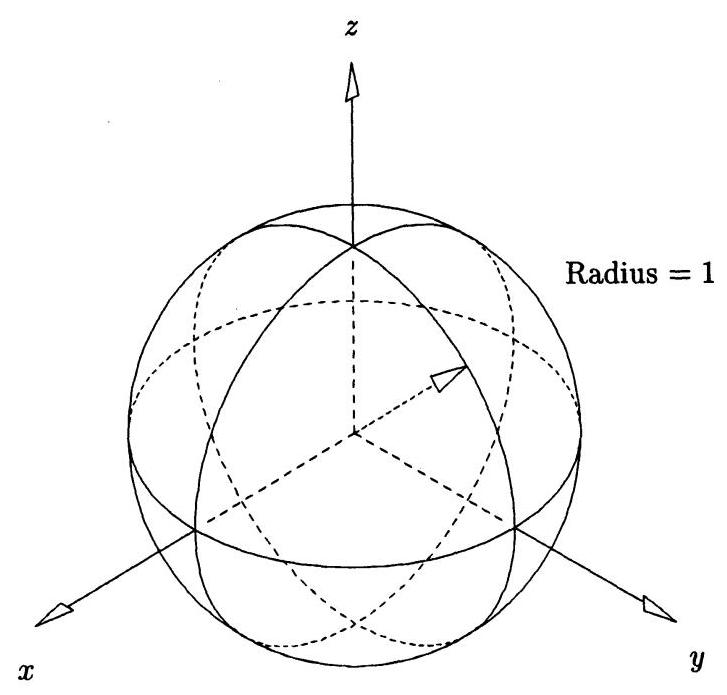
\includegraphics[max width=0.6\textwidth]{images/0193ba0d-ab19-7138-9798-cb281ce60de0_14_398_1393_727_695_0.jpg}
\end{center}
\hspace*{3em} 

图 1.3. 半径为 1 的球体，位于原点。

记 \(\mathbf{S}\left( {u,v}\right)\) 的偏导数为 \({\mathbf{S}}_{u}\left( {u,v}\right)  = \left( {{x}_{u}\left( {u,v}\right) ,{y}_{u}\left( {u,v}\right) }\right.\) 、 \(\left. {{z}_{u}\left( {u,v}\right) }\right)\) 和 \({\mathbf{S}}_{v}\left( {u,v}\right)  = \left( {{x}_{v}\left( {u,v}\right) ,{y}_{v}\left( {u,v}\right) ,{z}_{v}\left( {u,v}\right) }\right)\) ，即沿纬线和经线的速度。在表面上的任何一点，如果向量叉积 \({\mathbf{S}}_{u} \times  {\mathbf{S}}_{v}\) 不为零，则单位法向量 \(\mathbf{N}\) 由(图 1.4)给出。

\[
\mathbf{N} = \frac{{\mathbf{S}}_{u} \times  {\mathbf{S}}_{v}}{\left| {\mathbf{S}}_{u} \times  {\mathbf{S}}_{v}\right| } \tag{1.4}
\]

在某一点存在法向量及相应的切平面是表面的几何属性，与参数化无关。不同的参数化给出不同的偏导数，但方程 (1.4) 始终产生 \(\mathbf{N}\) ，前提是分母不为零。从方程 (1.3) 可以看出，对于所有 \(v,0 \leq  v \leq  {2\pi },{\mathbf{S}}_{v}\left( {0,v}\right)  = {\mathbf{S}}_{v}\left( {\pi ,v}\right)  = 0\) ，即 \({\mathbf{S}}_{v}\) 在球体的南北极消失。显然，在两个极点确实存在法向量，但在这种参数化下，方程 (1.4) 不能用于计算它们。

在隐式和参数化形式中，很难坚持认为其中一种形式总是比另一种更合适。两者各有优缺点。成功的几何建模使用了这两种技术。以下是两种方法的比较:

\begin{center}
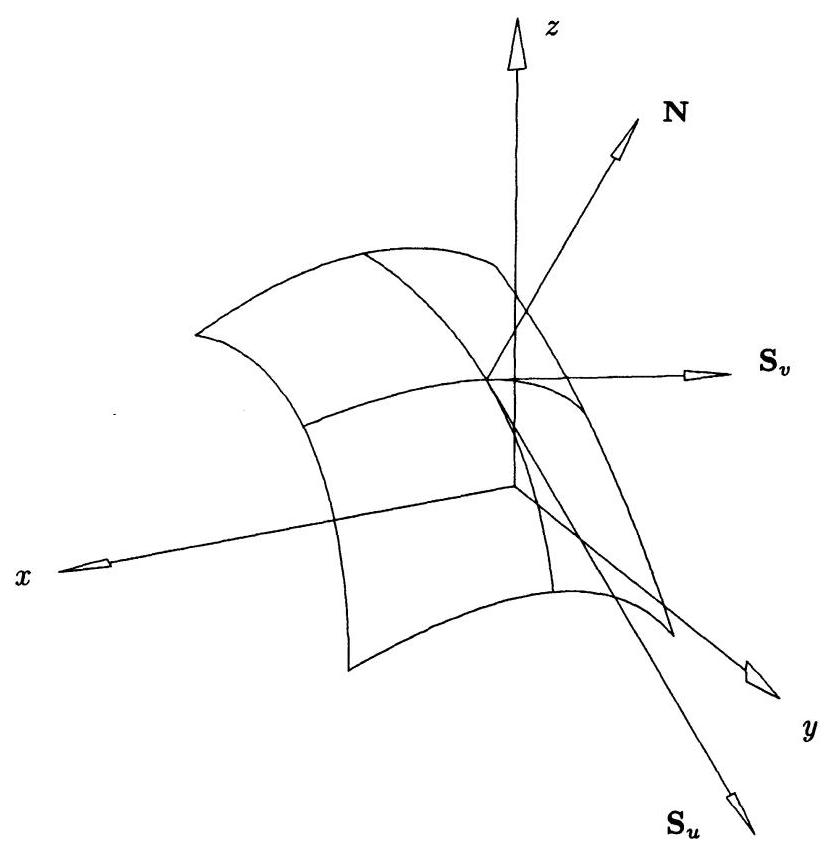
\includegraphics[max width=0.7\textwidth]{images/0193ba0d-ab19-7138-9798-cb281ce60de0_15_355_1217_827_848_0.jpg}
\end{center}
\hspace*{3em} 

图 1.4. \(\mathbf{S}\left( {u,v}\right)\) 的偏导数和单位法向量。

\begin{itemize}
\item 通过添加一个 \(z\) 坐标，参数化方法可以轻松扩展以表示三维空间中的任意曲线， \(\mathbf{C}\left( u\right)  = \left( {x\left( u\right) ,y\left( u\right) ,z\left( u\right) }\right)\) ；隐式形式仅指定 \({xy}\) (或 \({xz}\) 或 \({yz}\) )平面上的曲线；
\end{itemize}

\begin{itemize}
\item 使用隐式形式表示有界曲线段(或表面片段)是繁琐的。然而，有界性通过参数区间的界限内置于参数化形式中。另一方面，使用参数化几何实现无界几何(例如，由 \(f\left( {x,y}\right)  = {ax} +\)  \({by} + c = 0)\) 给出的简单直线)是困难的；
\end{itemize}

\begin{itemize}
\item 参数曲线具有自然的遍历方向(如果 \(a \leq  u \leq  b\) ，则从 \(\mathbf{C}\left( a\right)\) 到 \(\mathbf{C}\left( b\right)\) )；隐式曲线则没有。因此，沿着参数曲线生成有序点序列是容易的。类似的说法也适用于在表面上生成点网格；
\end{itemize}

\begin{itemize}
\item 参数形式在计算机中设计和表示形状时更为自然。许多参数函数的系数，例如，Bézier 和 B-spline，具有相当大的几何意义。这转化为直观的设计方法和具有明显几何特征的数值稳定算法；
\end{itemize}

\begin{itemize}
\item 许多几何操作和处理的复杂性在很大程度上取决于表示方法。两个经典的例子是:
\end{itemize}

\begin{itemize}
\item 计算曲线或表面上的一个点 - 在隐式形式中困难； - 给定一个点，确定它是否在曲线或表面上 - 在参数形式中困难；
\end{itemize}

\begin{itemize}
\item 在参数形式中，有时必须处理与真实几何无关的参数异常。一个例子是单位球体(见 Eq.[1.3])。极点是参数临界点，算法上难以处理，但在几何上，极点与球体上的任何其他点没有区别。
\end{itemize}

本书其余部分几乎完全关注参数形式。关于隐式和参数形式的更多细节可以在标准文献中找到([Faux81; Mort85; Hoff89; Beac91])。



\section{曲线的幂基形式}

显然，通过允许坐标函数 \(x\left( u\right) ,y\left( u\right)\) 和 \(z\left( u\right)\) 为任意，我们可以获得各种各样的曲线。然而，在实现几何建模系统时存在权衡。理想的情况是将自己限制在一类函数中，这些函数

\begin{itemize}
\item 能够精确表示系统用户所需的所有曲线；
\end{itemize}

\begin{itemize}
\item 在计算机中易于、高效且准确地处理，特别是:
\end{itemize}

\begin{itemize}
\item 曲线上的点和导数的计算是高效的；
\end{itemize}

\begin{itemize}
\item 函数的数值处理对浮点舍入误差相对不敏感；
\end{itemize}

\begin{itemize}
\item 这些函数对存储的内存要求很少；
\end{itemize}

\begin{itemize}
\item 简单且在数学上被很好地理解。
\end{itemize}

一类广泛使用的函数是多项式。尽管它们满足此列表中的最后两个标准，但仍有许多重要的曲线(和表面)类型无法通过多项式精确表示；这些曲线必须在使用多项式的系统中进行近似。在本节及下一节中，我们研究表达多项式函数的两种常见方法:幂基和贝塞尔。尽管在数学上是等价的，但我们将看到贝塞尔方法更适合在计算机中表示和操作形状。

一个 \(n\) 次幂基曲线由以下公式给出

\[
\mathbf{C}\left( u\right)  = \left( {x\left( u\right) ,y\left( u\right) ,z\left( u\right) }\right)  = \mathop{\sum }\limits_{{i = 0}}^{n}{\mathbf{a}}_{i}{u}^{i}\;0 \leq  u \leq  1 \tag{1.5}
\]

\({\mathbf{a}}_{i} = \left( {{x}_{i},{y}_{i},{z}_{i}}\right)\) 是向量，因此

\[
x\left( u\right)  = \mathop{\sum }\limits_{{i = 0}}^{n}{x}_{i}{u}^{i}\;y\left( u\right)  = \mathop{\sum }\limits_{{i = 0}}^{n}{y}_{i}{u}^{i}\;z\left( u\right)  = \mathop{\sum }\limits_{{i = 0}}^{n}{z}_{i}{u}^{i}
\]

在矩阵形式下，方程(1.5)为

\[
\mathbf{C}\left( u\right)  = \left\lbrack  \begin{array}{llll} {\mathbf{a}}_{0} & {\mathbf{a}}_{1} & \cdots & {\mathbf{a}}_{n} \end{array}\right\rbrack  \left\lbrack  \begin{matrix} 1 \\  u \\  \vdots \\  {u}^{n} \end{matrix}\right\rbrack   = {\left\lbrack  {\mathbf{a}}_{i}\right\rbrack  }^{T}\left\lbrack  {u}^{i}\right\rbrack   \tag{1.6}
\]

(我们将行向量写作列向量的转置。)

对方程(1.5)进行微分得到

\[
{\mathbf{a}}_{i} = \frac{{\mathbf{C}}^{\left( i\right) }\left( u\right) { \mid  }_{u = 0}}{i!}
\]

其中 \({\left. {\mathbf{C}}^{\left( i\right) }\left( u\right) \right| }_{u = 0}\) 是 \(i\) 在 \(u = 0\) 处的 \(\mathbf{C}\left( u\right)\) 次导数。 \(n + 1\) 函数 \(\left\{  {u}^{i}\right\}\) 被称为基函数(或混合函数)，而 \(\left\{  {\mathbf{a}}_{i}\right\}\) 是幂基表示的系数。

给定 \({u}_{0}\) ，在幂基曲线上的点 \(\mathbf{C}\left( {u}_{0}\right)\) 最有效的计算方法是使用霍纳法

\begin{itemize}
\item 对于 \(= 1 : \mathbf{C}\left( {u}_{0}\right)  = {\mathbf{a}}_{1}{u}_{0} + {\mathbf{a}}_{0}\) 次
\end{itemize}

\begin{itemize}
\item 学位 \(= 2 : \mathbf{C}\left( {u}_{0}\right)  = \left( {{\mathbf{a}}_{2}{u}_{0} + {\mathbf{a}}_{1}}\right) {u}_{0} + {\mathbf{a}}_{0}\)
\end{itemize}

. :

\[
\text{ degree } = \mathrm{n} : \mathbf{C}\left( {u}_{0}\right)  = \left( {\left( {\cdots \left( {{\mathbf{a}}_{n}{u}_{0} + {\mathbf{a}}_{n - 1}}\right) {u}_{0} + {\mathbf{a}}_{n - 2}}\right) {u}_{0} + \cdots  + {\mathbf{a}}_{0}}\right.
\]

一般算法是

\HRule

ALGORITHM A1.1

\hspace*{2em} Horner1(a, n, u0, C)

\hspace*{4em} \{ /* Compute point on power basis curve. */

\hspace*{7em} /* Input: a, n, u0 */

\hspace*{7em} /* Output: C */

\hspace*{4em} C = a[n];

\hspace*{4em} for (i=n-1; i>=0; i--)

\hspace*{6em} C = C*u0 + a[i];

\hspace*{3em} \}

\HRule

\section*{示例}

Ex1.1 \(n = 1\) 。 \(\mathbf{C}\left( u\right)  = {\mathbf{a}}_{0} + {\mathbf{a}}_{1}u,0 \leq  u \leq  1\) 是连接点 \({\mathbf{a}}_{0}\) 和 \({\mathbf{a}}_{0} + {\mathbf{a}}_{1}\) 的直线段(图 1.5)。常数 \({\mathbf{C}}^{\prime }\left( u\right)  = {\mathbf{a}}_{1}\) 给出了线的方向。

Ex1.2 \(n = 2\) 。一般来说， \(\mathbf{C}\left( u\right)  = {\mathbf{a}}_{0} + {\mathbf{a}}_{1}u + {\mathbf{a}}_{2}{u}^{2},0 \leq  u \leq  1\) 是连接点 \({\mathbf{a}}_{0}\) 和 \({\mathbf{a}}_{0} + {\mathbf{a}}_{1} + {\mathbf{a}}_{2}\) 的抛物线弧(图 1.6)。这可以通过以下方式显示:

1. 将 \(\mathbf{C}\left( u\right)\) 变换到 \({xy}\) 平面( \(\mathbf{C}\left( u\right)\) 确实位于一个唯一的平面内)；

2. 设定 \(x = {x}_{0} + {x}_{1}u + {x}_{2}{u}^{2}\) 和 \(y = {y}_{0} + {y}_{1}u + {y}_{2}{u}^{2}\) ，然后从这些方程中消去 \(u\) 和 \({u}^{2}\) ，以获得关于 \(x\) 和 \(y\) 的二次隐式方程；

3. 观察隐式方程的形式是抛物线的形式。

注意，加速度向量 \({\mathbf{C}}^{\prime \prime }\left( u\right)  = 2{\mathbf{a}}_{2}\) 是一个常量。有两个特殊的(退化的)情况值得关注，均发生在向量 \({\mathbf{a}}_{2}\) 与初始切向量 \({\mathbf{a}}_{1}\) 平行时(当 \({x}_{1}{y}_{2} = {x}_{2}{y}_{1}\) 时)。在这种情况下，切向量不转动，即我们得到一条直线。向量 \({a}_{2}\) 可以指向与 \({a}_{1}\) 相同的方向(图 1.7a)，或指向相反的方向(图 1.7b)。在图 \({1.7}\mathrm{\;b},{\mathrm{a}}_{1} + 2{\mathrm{a}}_{2}{u}_{0} = 0\) 中，对于某些 \(0 \leq  {u}_{0} \leq  1\) (速度趋于零，粒子停止)，线段的一部分在相反方向上被重新追踪。

\begin{center}
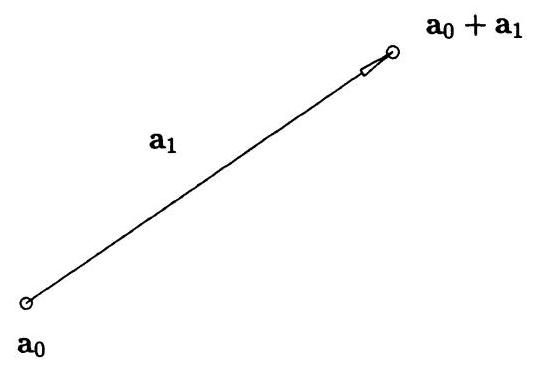
\includegraphics[max width=0.4\textwidth]{images/0193ba0d-ab19-7138-9798-cb281ce60de0_18_154_1785_533_376_0.jpg}
\end{center}
\hspace*{3em} 

图 1.5. 直线段， \(\mathbf{C}\left( u\right)  = {\mathbf{a}}_{0} + {\mathbf{a}}_{1}u\)

\begin{center}
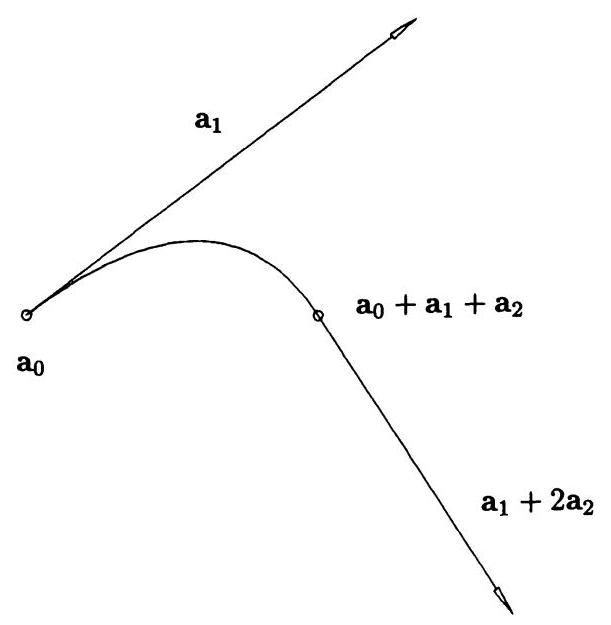
\includegraphics[max width=0.5\textwidth]{images/0193ba0d-ab19-7138-9798-cb281ce60de0_19_468_273_611_625_0.jpg}
\end{center}
\hspace*{3em} 

图 1.6. 抛物线弧， \(\mathbf{C}\left( u\right)  = {\mathbf{a}}_{0} + {\mathbf{a}}_{1}u + {\mathbf{a}}_{2}{u}^{2}\) 。

Ex1.3 \(n = 3\) 。三次曲线 \(\mathbf{C}\left( u\right)  = {\mathbf{a}}_{0} + {\mathbf{a}}_{1}u + {\mathbf{a}}_{2}{u}^{2} + {\mathbf{a}}_{3}{u}^{3}\) 是一种非常一般的曲线；它可以是一个真正扭曲的三维曲线，不在同一平面内(图 1.8a)；它可以有一个拐点(图 1.8b)；一个尖点(图 1.8c)；或一个环(图 1.8d)。如果 \({\mathbf{a}}_{0},{\mathbf{a}}_{1},{\mathbf{a}}_{2},{\mathbf{a}}_{3}\) 不在唯一平面内，则会产生扭曲曲线。平面曲线上的拐点被定义为曲线光滑(没有尖点)且该点的切线通过曲线的点。这意味着曲线的转向方向发生了变化。在拐点处，要么 \({\mathbf{C}}^{\prime \prime }\left( u\right)  = 0\) ，要么 \({\mathbf{C}}^{\prime }\left( u\right)  ⫫ {\mathbf{C}}^{\prime \prime }\left( u\right)\) 。在 \(u = {u}_{0}\) 处形成尖点的必要(但不充分)条件是 \({\mathbf{C}}^{\prime }\left( {u}_{0}\right)  = 0\) (速度为零)。环出现的条件也已知(见 [Ferg66, 67, 69, 93; Forr70, 80; Wang81; Ston89; Su89])。

\begin{center}
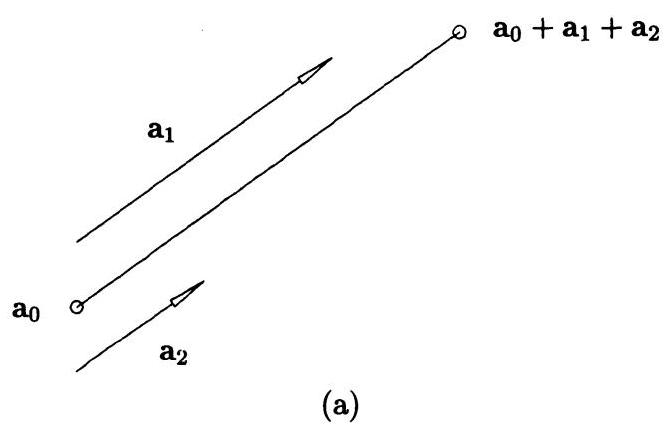
\includegraphics[max width=0.6\textwidth]{images/0193ba0d-ab19-7138-9798-cb281ce60de0_19_433_1673_668_431_0.jpg}
\end{center}
\hspace*{3em} 

图 1.7. \({\mathbf{a}}_{1}\) 和 \({\mathbf{a}}_{2}\) 平行。 (a) 同一方向；(b) 相反方向。

\begin{center}
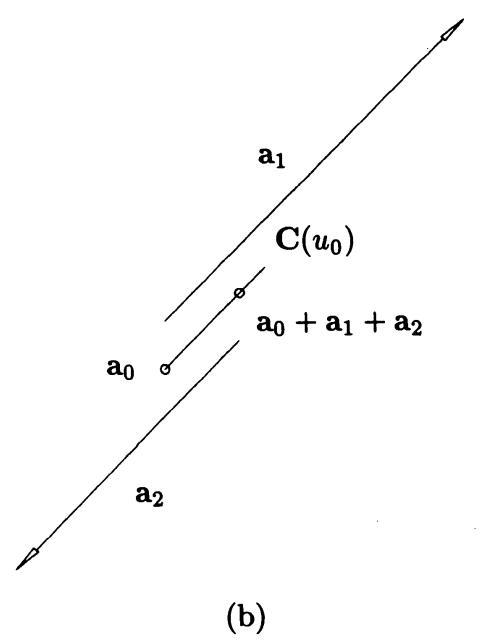
\includegraphics[max width=0.4\textwidth]{images/0193ba0d-ab19-7138-9798-cb281ce60de0_20_528_280_481_643_0.jpg}
\end{center}
\hspace*{3em} 

图 1.7. (续。)

\section{Bézier 曲线}

接下来我们研究另一种参数多项式曲线，贝塞尔曲线。由于它们都使用多项式作为坐标函数，幂基和贝塞尔形式在数学上是等价的；即，任何可以用一种形式表示的曲线也可以用另一种形式表示。然而，贝塞尔方法在几何建模方面优于幂基形式。我们对贝塞尔曲线的介绍相对非正式；对于更严格和完整的处理，读者应参考其他文献 [Forr72; Bezi72, 86; Gord74a; Chan81; Fari93; Yama88; Hosc93; Roge90]。

幂基形式有以下缺点:

\begin{itemize}
\item 对于交互式形状设计来说不自然；系数 \(\left\{  {\mathbf{a}}_{i}\right\}\) 对曲线形状的几何洞察力非常有限。此外，设计师通常希望在曲线的两端指定边界条件，而不仅仅是在起始点；
\end{itemize}

\begin{itemize}
\item 处理幂基多项式的算法具有代数而非几何的特征(例如，霍纳法则)；
\end{itemize}

\begin{itemize}
\item 在数值上，它是一种相对较差的形式；例如，当系数的大小差异很大时，霍纳法则容易产生舍入误差(参见 [Faro87, 88; Dani89])。
\end{itemize}

贝塞尔方法弥补了这些缺点。

一个 \(n\) 次贝塞尔曲线定义为

\[
\mathbf{C}\left( u\right)  = \mathop{\sum }\limits_{{i = 0}}^{n}{B}_{i,n}\left( u\right) {\mathbf{P}}_{i}\;0 \leq  u \leq  1 \tag{1.7}
\]

\begin{center}
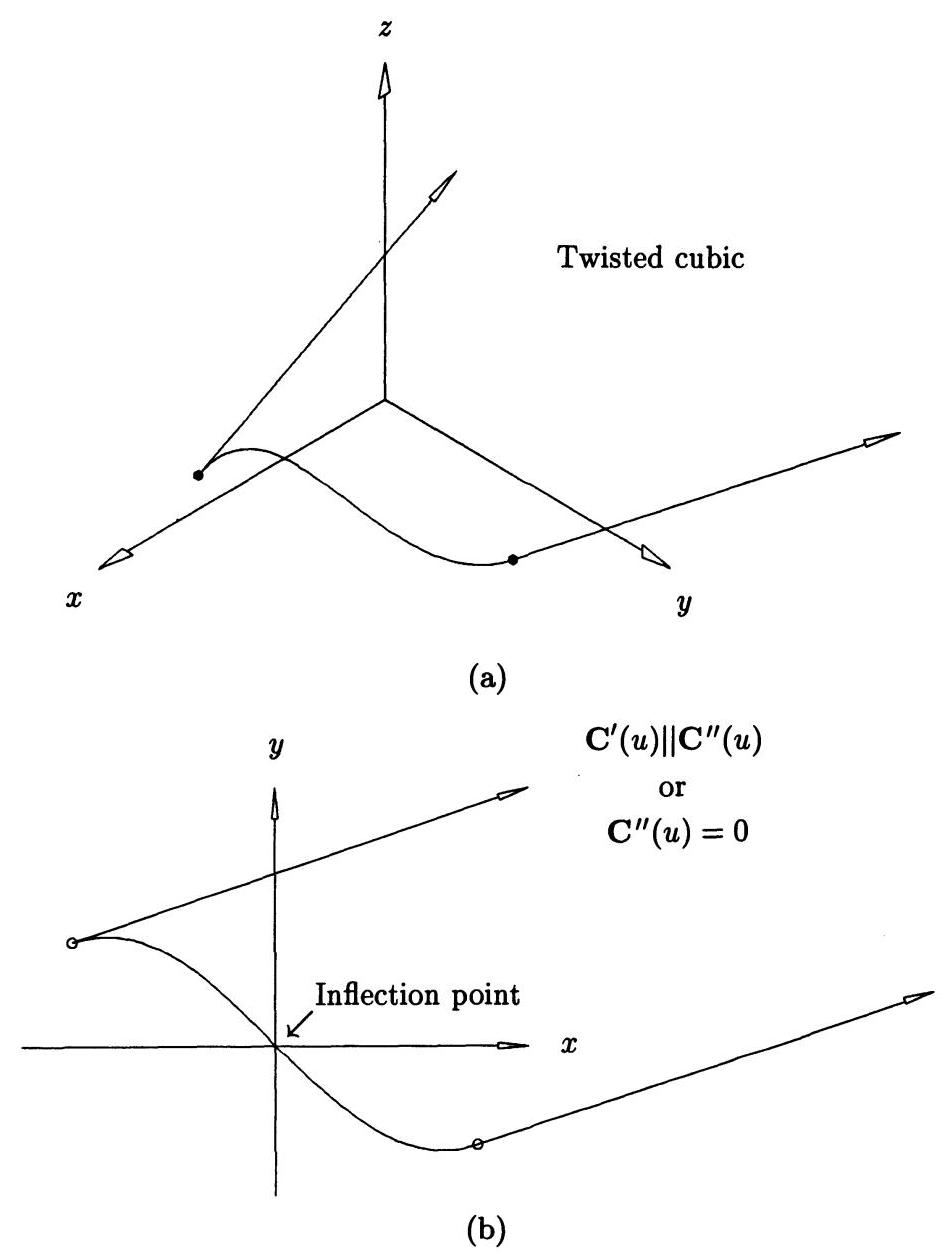
\includegraphics[max width=0.8\textwidth]{images/0193ba0d-ab19-7138-9798-cb281ce60de0_21_291_257_952_1256_0.jpg}
\end{center}
\hspace*{3em} 

图 1.8. 三次曲线。(a)三维扭曲；(b)拐点；(c)尖点；(d)环。

基函数(混合函数) \(\left\{  {{B}_{i,n}\left( u\right) }\right\}\) 是经典的 \(n\) 次伯恩斯坦多项式 ([Bern12; Lore86])，其表达式为

\[
{B}_{i,n}\left( u\right)  = \frac{n!}{i!\left( {n - i}\right) !}{u}^{i}{\left( 1 - u\right) }^{n - i} \tag{1.8}
\]

这种形式的几何系数 \(\left\{  {\mathbf{P}}_{i}\right\}\) 被称为控制点。注意，定义 Eq. (1.7) 要求 \(u \in  \left\lbrack  {0,1}\right\rbrack\) 。

\section*{示例}

Ex1.4 \(n = 1\) 。根据公式 (1.8)，我们有 \({B}_{0,1}\left( u\right)  = 1 - u\) 和 \({B}_{1,1}\left( u\right)  = u\) ；而公式 (1.7) 的形式为 \(\mathbf{C}\left( u\right)  = \left( {1 - u}\right) {\mathbf{P}}_{0} + u{\mathbf{P}}_{1}\) 。这是从 \({\mathbf{P}}_{0}\) 到 \({\mathbf{P}}_{1}\) 的一条直线段(见图 1.9)。

\begin{center}
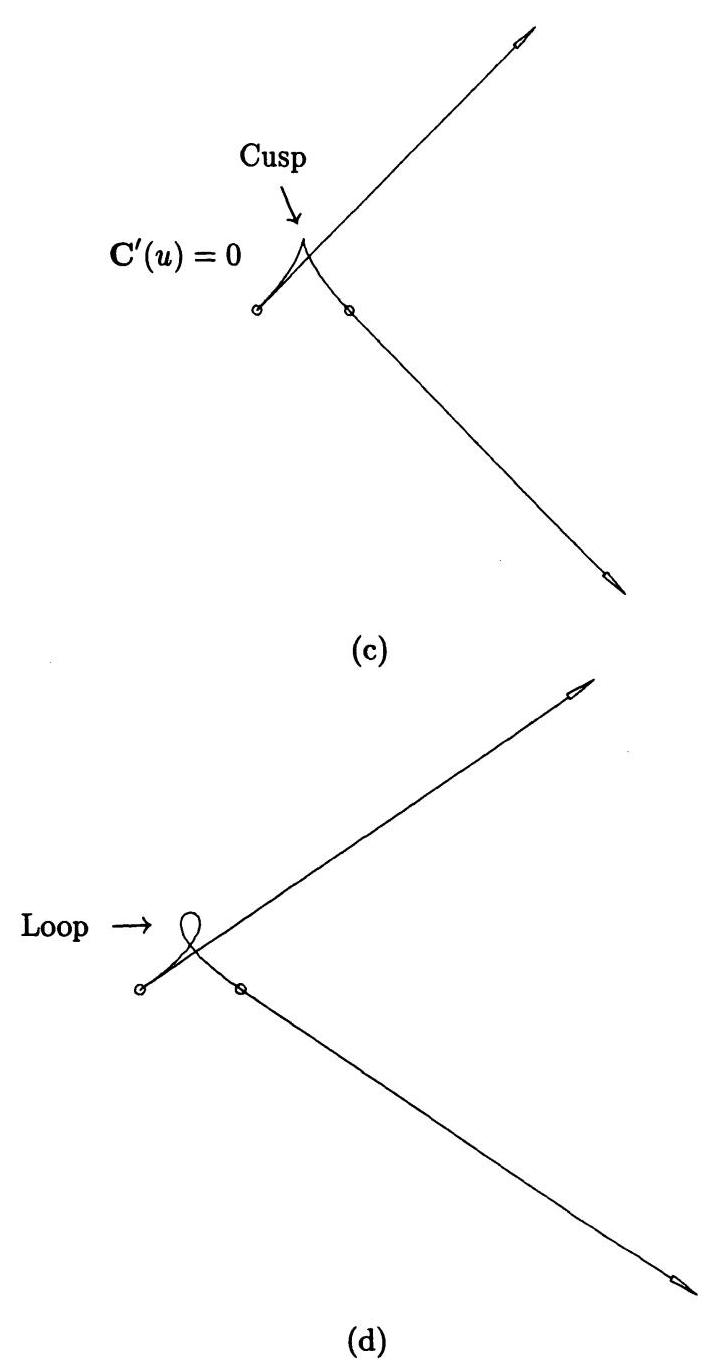
\includegraphics[max width=0.6\textwidth]{images/0193ba0d-ab19-7138-9798-cb281ce60de0_22_406_241_706_1369_0.jpg}
\end{center}
\hspace*{3em} 

图 1.8. (续)

Ex1.5 \(n = 2\) 。根据公式 (1.7) 和 (1.8)，我们有 \(\mathbf{C}\left( u\right)  = {\left( 1 - u\right) }^{2}{\mathbf{P}}_{0} +\)  \({2u}\left( {1 - u}\right) {\mathbf{P}}_{1} + {u}^{2}{\mathbf{P}}_{2}\) 。这是从 \({\mathbf{P}}_{0}\) 到 \({\mathbf{P}}_{2}\) 的一条抛物线弧(见图 1.10)。注意到

\begin{itemize}
\item 由 \(\left\{  {{\mathbf{P}}_{0},{\mathbf{P}}_{1},{\mathbf{P}}_{2}}\right\}\) 形成的多边形，称为控制多边形，较好地近似了曲线的形状；
\end{itemize}

\begin{itemize}
\item \({\mathbf{P}}_{0} = \mathbf{C}\left( 0\right)\) 和 \({\mathbf{P}}_{2} = \mathbf{C}\left( 1\right)\) ；
\end{itemize}

\begin{itemize}
\item 曲线在其端点的切线方向与 \({\mathbf{P}}_{1} - {\mathbf{P}}_{0}\) 和 \({\mathbf{P}}_{2} - {\mathbf{P}}_{1}\) 平行(这一点将在后面推导)；
\end{itemize}

\begin{itemize}
\item 曲线包含在由 \({\mathbf{P}}_{0}{\mathbf{P}}_{1}{\mathbf{P}}_{2}\) 形成的三角形内。
\end{itemize}

\begin{center}
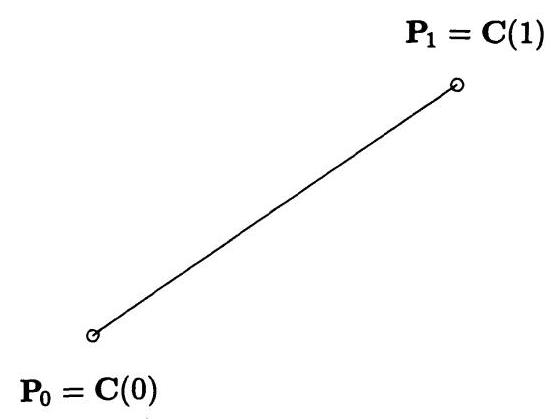
\includegraphics[max width=0.5\textwidth]{images/0193ba0d-ab19-7138-9798-cb281ce60de0_23_487_276_555_419_0.jpg}
\end{center}
\hspace*{3em} 

图 1.9. 一阶 Bézier 曲线。

Ex \({1.6n} = 3\) 。我们有 \(\mathbf{C}\left( u\right)  = {\left( 1 - u\right) }^{3}{\mathbf{P}}_{0} + {3u}{\left( 1 - u\right) }^{2}{\mathbf{P}}_{1} + 3{u}^{2}\left( {1 - u}\right) {\mathbf{P}}_{2} + {u}^{3}{\mathbf{P}}_{3}\) 。立方 Bézier 曲线的例子见图 1.11a 至 1.11f。注意到

\begin{itemize}
\item 控制多边形近似了曲线的形状；
\end{itemize}

\begin{itemize}
\item \({\mathbf{P}}_{0} = \mathbf{C}\left( 0\right)\) 和 \({\mathbf{P}}_{3} = \mathbf{C}\left( 1\right)\) ；
\end{itemize}

\begin{itemize}
\item 端点切线方向与 \({\mathbf{P}}_{1} - {\mathbf{P}}_{0}\) 和 \({\mathbf{P}}_{3} - {\mathbf{P}}_{2}\) 平行；
\end{itemize}

\begin{itemize}
\item 凸包性质:曲线包含在其定义控制点的凸包内(图 1.11c)；
\end{itemize}

\begin{itemize}
\item 变差减少性质:没有直线与曲线相交的次数超过它与曲线的控制多边形相交的次数(对于三维 Bézier 曲线，将“直线”替换为
\end{itemize}

\begin{center}
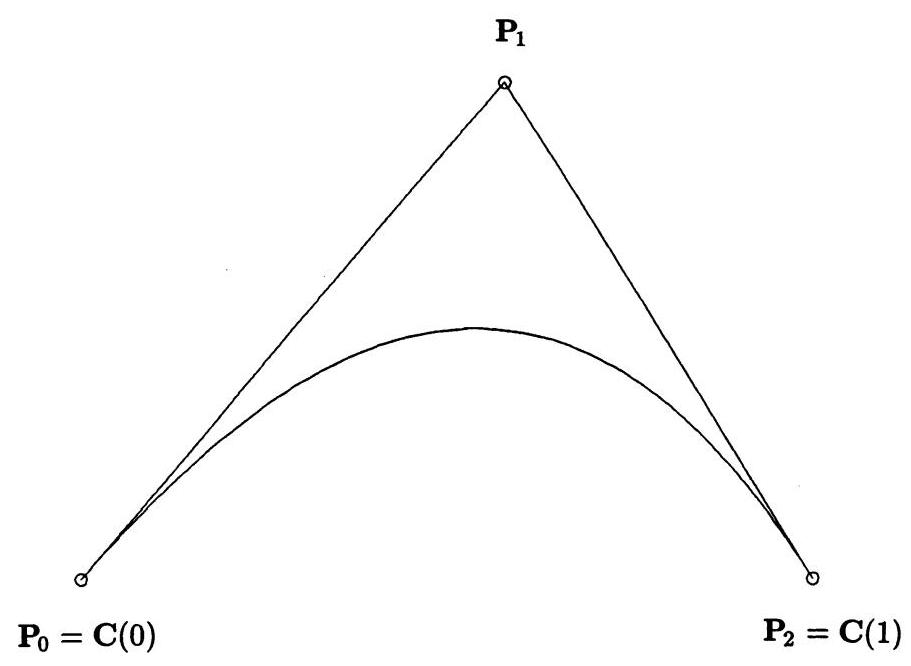
\includegraphics[max width=0.8\textwidth]{images/0193ba0d-ab19-7138-9798-cb281ce60de0_23_311_1427_911_666_0.jpg}
\end{center}
\hspace*{3em} 

图 1.10. 二次贝塞尔曲线。

\begin{center}
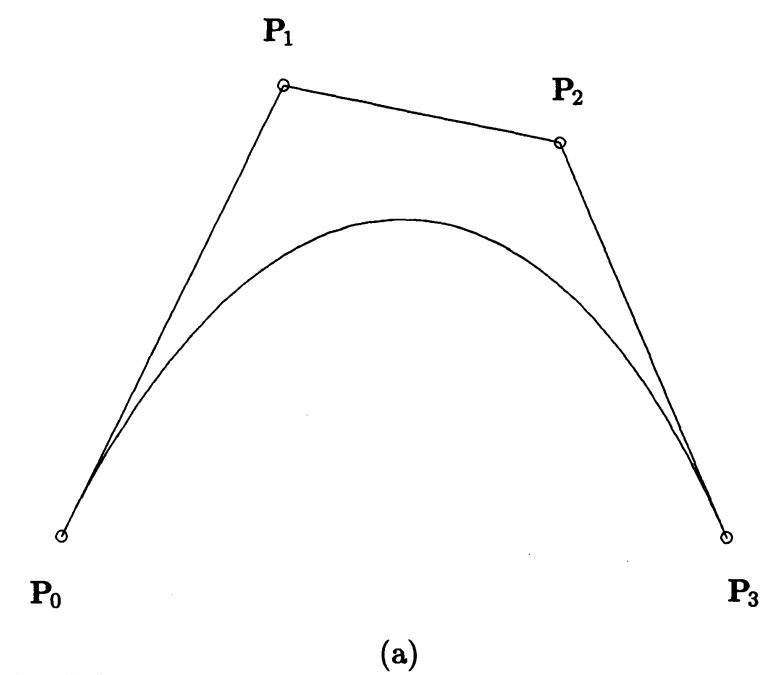
\includegraphics[max width=0.7\textwidth]{images/0193ba0d-ab19-7138-9798-cb281ce60de0_24_376_248_774_675_0.jpg}
\end{center}
\hspace*{3em} 

图 1.11. 三次贝塞尔曲线。

单词“平面”。这表达了贝塞尔曲线紧密跟随其控制多边形的特性，并且不会比其控制多边形更大幅度地摆动(图 1.11f)；

\begin{itemize}
\item 最初(在 \(u = 0\) 时)曲线的转向与 \({\mathbf{P}}_{0}{\mathbf{P}}_{1}{\mathbf{P}}_{2}\) 相同。在 \(u = 1\) 时，它的转向为 \({\mathbf{P}}_{1}{\mathbf{P}}_{2}{\mathbf{P}}_{3}\) ；
\end{itemize}

\begin{itemize}
\item 控制多边形中的环可能暗示曲线中的环，也可能不暗示。从图 1.11e 到图 1.11f 的过渡是一个具有尖点的曲线。
\end{itemize}

\begin{center}
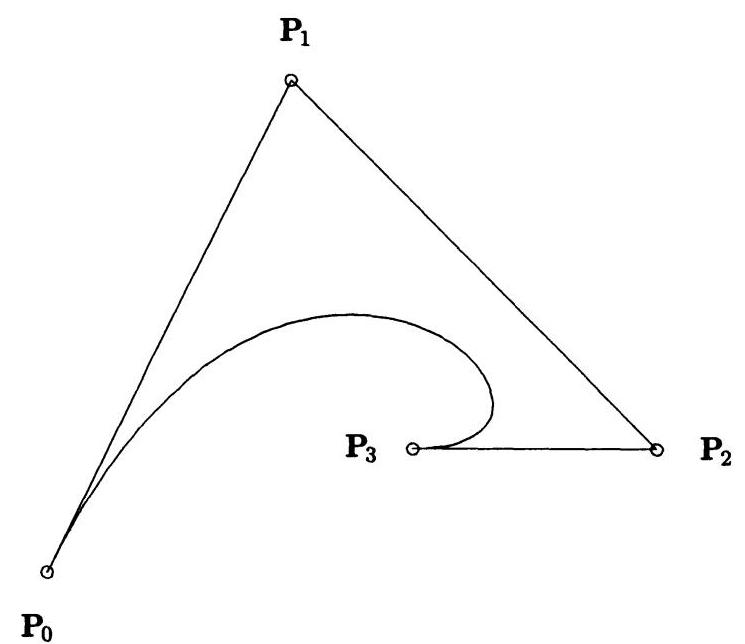
\includegraphics[max width=0.6\textwidth]{images/0193ba0d-ab19-7138-9798-cb281ce60de0_24_395_1427_745_644_0.jpg}
\end{center}
\hspace*{3em} 

图 1.11. (续)

14 曲线和曲面基础

\begin{center}
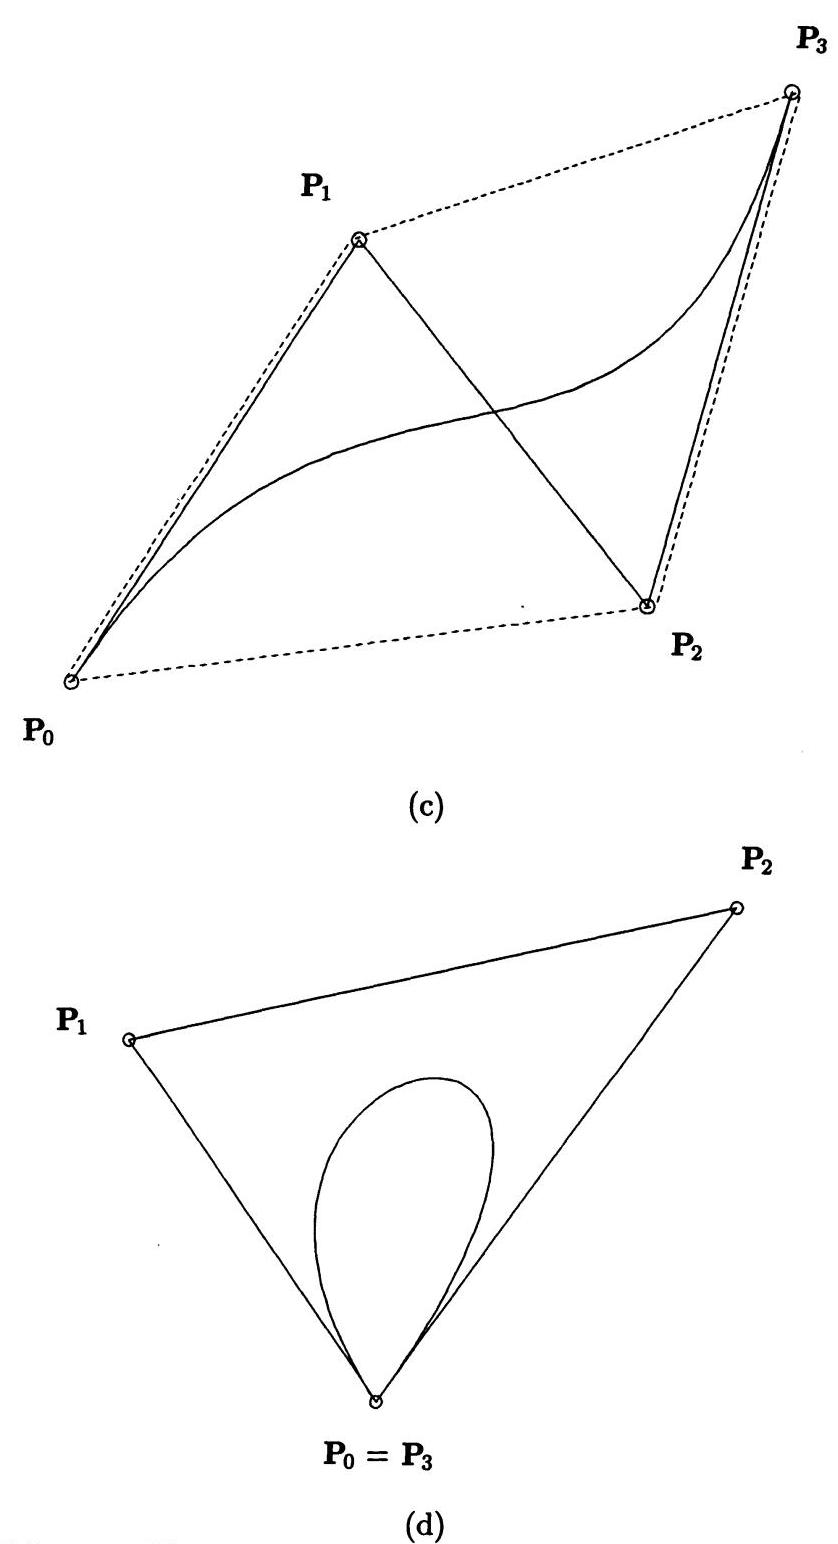
\includegraphics[max width=0.7\textwidth]{images/0193ba0d-ab19-7138-9798-cb281ce60de0_25_351_269_838_1544_0.jpg}
\end{center}
\hspace*{3em} 

图 1.11. (续)

Ex1.7 \(n = 6\) 。图 1.12 显示了一个六次闭合的 Bézier 曲线。由于 \({\mathbf{P}}_{1} - {\mathbf{P}}_{0}\) 与 \({\mathbf{P}}_{6} - {\mathbf{P}}_{5}\) 平行，该曲线在 \(\mathbf{C}\left( 0\right) \left( { = \mathbf{C}\left( 1\right) }\right)\) 处是光滑的。我们所说的光滑是指在 \(u = 0\) 和 \(u = 1\) 处的切向量具有相同的方向。

除了前面提到的性质外，Bézier 曲线在旋转、平移和缩放等常见变换下是不变的；也就是说，通过对控制多边形应用变换来对曲线应用变换。我们将在第 3 章中更严格地介绍这个概念，针对 B-spline 曲线(Bézier 曲线是其特例)。

\begin{center}
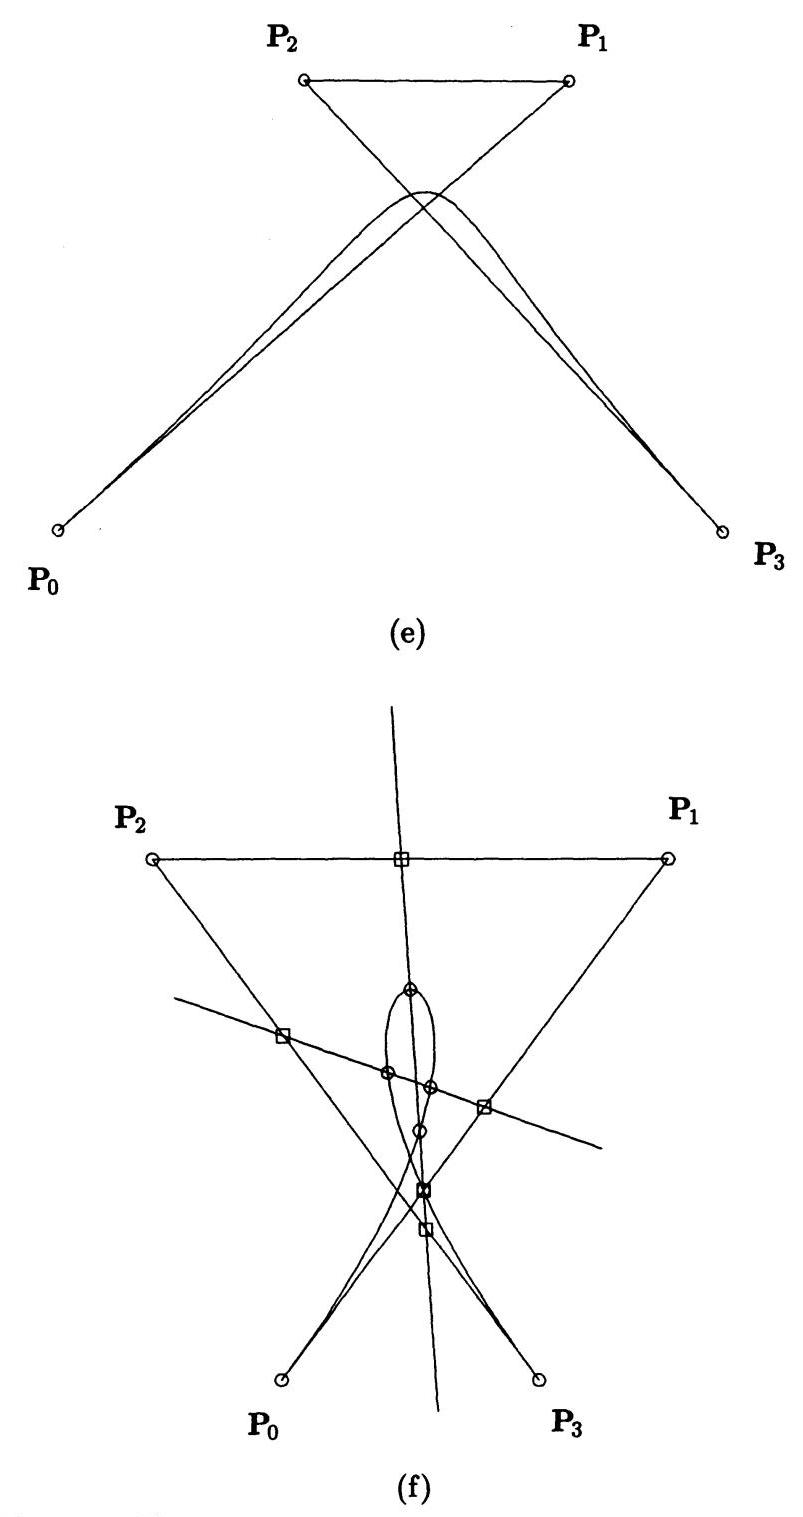
\includegraphics[max width=0.7\textwidth]{images/0193ba0d-ab19-7138-9798-cb281ce60de0_26_361_248_803_1517_0.jpg}
\end{center}
\hspace*{3em} 

图 1.11. (续。)

在任何曲线(或曲面)表示方案中，基函数的选择决定了该方案的几何特性。图 \({1.13}\mathrm{a} - \mathrm{d}\) 显示了 \(\left\{  {{B}_{i,n}\left( u\right) }\right\}\) 的基函数 \(n = 1,2,3,9\) 。这些函数具有以下性质:

P1.1 非负性:对于所有 \(i,n\) 和 \(0 \leq  u \leq  1\) ，有 \({B}_{i,n}\left( u\right)  \geq  0\) ；

16 曲线与曲面基础

\begin{center}
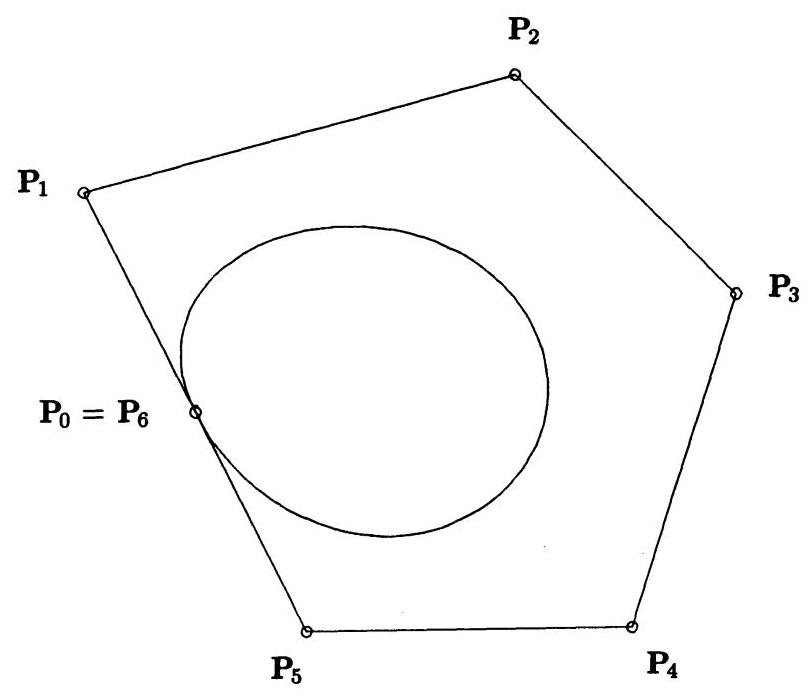
\includegraphics[max width=0.7\textwidth]{images/0193ba0d-ab19-7138-9798-cb281ce60de0_27_362_254_811_696_0.jpg}
\end{center}
\hspace*{3em} 

图 1.12. 一个光滑的闭合六次 Bézier 曲线。

P1.2 单位分割:对于所有 \(0 \leq  u \leq  1\) ，有 \(\mathop{\sum }\limits_{{i = 0}}^{n}{B}_{i,n}\left( u\right)  = 1\) ；

P1. \(3{B}_{0,n}\left( 0\right)  = {B}_{n,n}\left( 1\right)  = 1\) ;

P1.4 \({B}_{i,n}\left( u\right)\) 在区间 \(\left\lbrack  {0,1}\right\rbrack\) 上恰好达到一个最大值，即在 \(u = i/n\) 处。

P1.5 对称性:对于任何 \(n\) ，多项式集合 \(\left\{  {{B}_{i,n}\left( u\right) }\right\}\) 关于 \(u = 1/2\) 是对称的；

\begin{center}
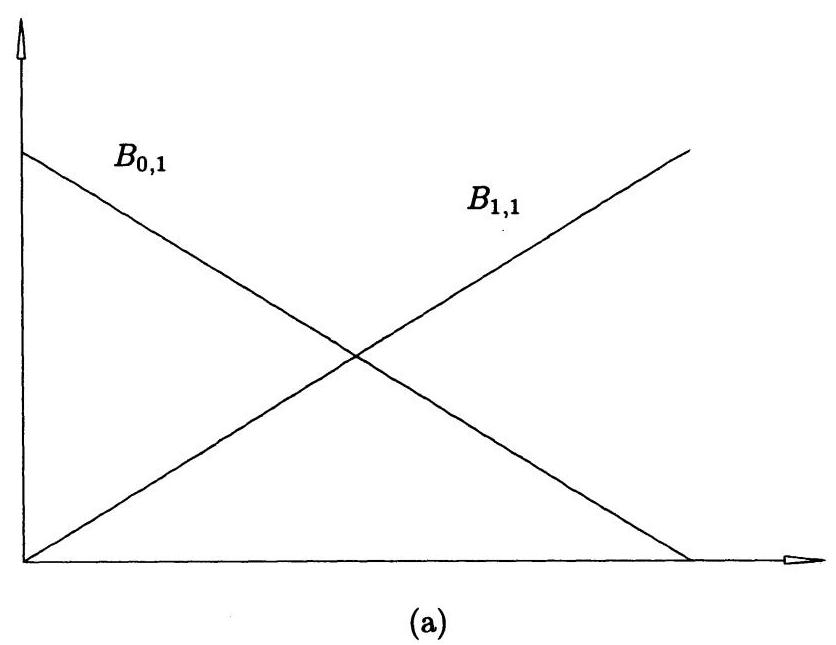
\includegraphics[max width=0.7\textwidth]{images/0193ba0d-ab19-7138-9798-cb281ce60de0_27_348_1468_836_645_0.jpg}
\end{center}
\hspace*{3em} 

图 1.13. 伯恩斯坦多项式(a) \(n = 1;\left( b\right) \mathrm{n} = 2;\left( \mathrm{c}\right) n = 3;\left( d\right) \mathrm{n} = 9\) 。

\begin{center}
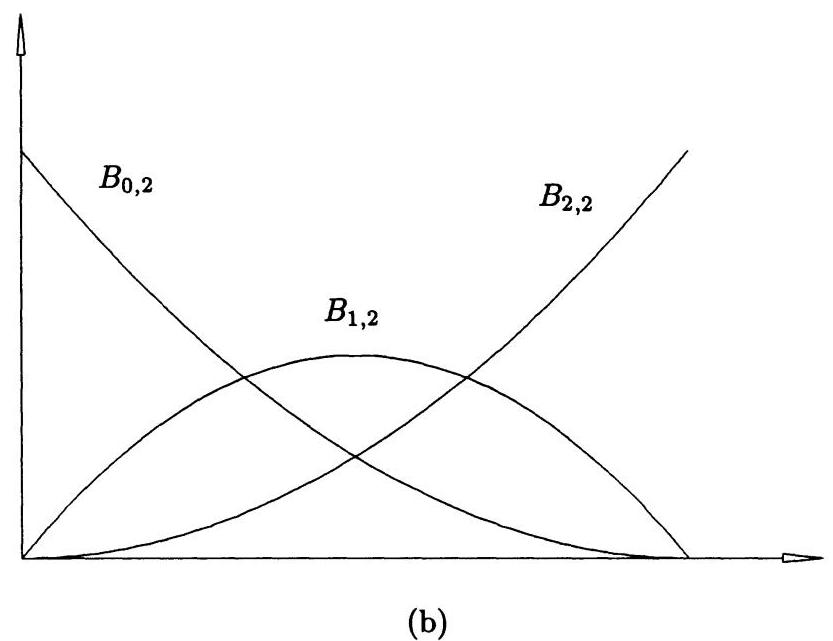
\includegraphics[max width=0.7\textwidth]{images/0193ba0d-ab19-7138-9798-cb281ce60de0_28_347_268_833_641_0.jpg}
\end{center}
\hspace*{3em} 

图 1.13. (续)

P1.6 递归定义: \({B}_{i,n}\left( u\right)  = \left( {1 - u}\right) {B}_{i,n - 1}\left( u\right)  + u{B}_{i - 1,n - 1}\left( u\right)\) (见图 1.14)；我们定义 \({B}_{i,n}\left( u\right)  \equiv  0\) 如果 \(i < 0\) 或 \(i > n\) ；

P1.7 导数:

\[
{B}_{i,n}^{\prime }\left( u\right)  = \frac{d{B}_{i,n}\left( u\right) }{du} = n\left( {{B}_{i - 1,n - 1}\left( u\right)  - {B}_{i,n - 1}\left( u\right) }\right)
\]

与

\[
{B}_{-1,n - 1}\left( u\right)  \equiv  {B}_{n,n - 1}\left( u\right)  \equiv  0
\]

图 1.15a 显示了 \({B}_{2,5}^{\prime }\) 的定义，而图 \({1.15}\mathrm{\;b}\) 则说明了所有的三次导数函数。18 曲线与曲面基础

\begin{center}
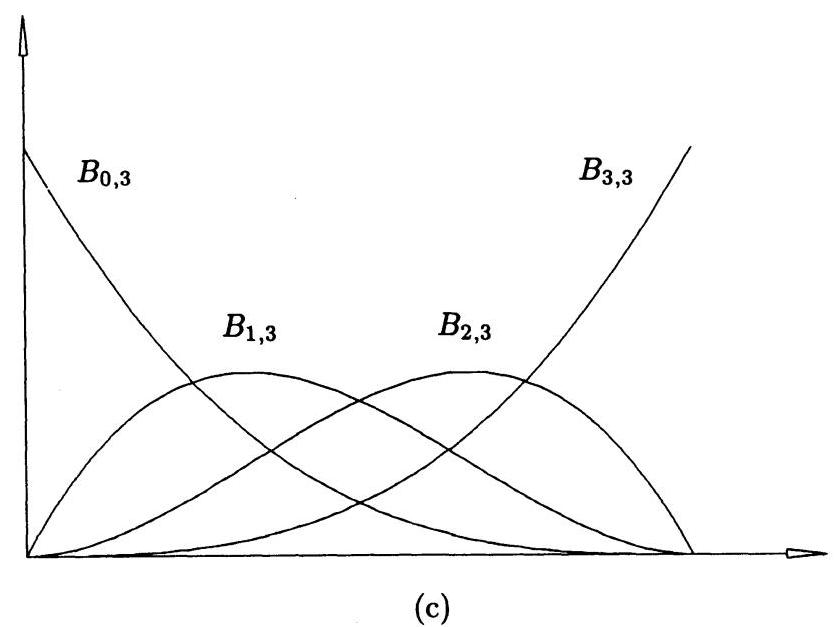
\includegraphics[max width=0.7\textwidth]{images/0193ba0d-ab19-7138-9798-cb281ce60de0_28_343_1505_838_627_0.jpg}
\end{center}
\hspace*{3em} 

图 1.13. (续)

\begin{center}
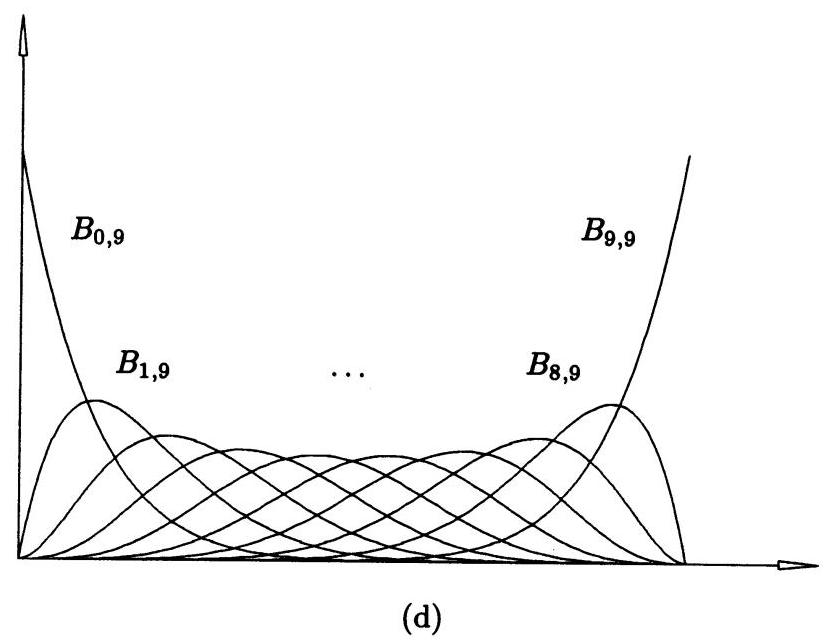
\includegraphics[max width=0.7\textwidth]{images/0193ba0d-ab19-7138-9798-cb281ce60de0_29_362_257_829_641_0.jpg}
\end{center}
\hspace*{3em} 

图 1.13. (续)

从方程 (1.8) 我们得到 \({B}_{0,0}\left( u\right)  = 1\) 。利用性质 P1.6，线性和二次 Bernstein 多项式为

\[
{B}_{0,1}\left( u\right)  = \left( {1 - u}\right) {B}_{0,0}\left( u\right)  + u{B}_{-1,0}\left( u\right)  = 1 - u
\]

\[
{B}_{1,1}\left( u\right)  = \left( {1 - u}\right) {B}_{1,0}\left( u\right)  + u{B}_{0,0}\left( u\right)  = u
\]

\[
{B}_{0,2}\left( u\right)  = \left( {1 - u}\right) {B}_{0,1}\left( u\right)  + u{B}_{-1,1}\left( u\right)  = {\left( 1 - u\right) }^{2}
\]

\[
{B}_{1,2}\left( u\right)  = \left( {1 - u}\right) {B}_{1,1}\left( u\right)  + u{B}_{0,1}\left( u\right)  = \left( {1 - u}\right) u + u\left( {1 - u}\right)  = {2u}\left( {1 - u}\right)
\]

\[
{B}_{2,2}\left( u\right)  = \left( {1 - u}\right) {B}_{2,1}\left( u\right)  + u{B}_{1,1}\left( u\right)  = {u}^{2}
\]

\begin{center}
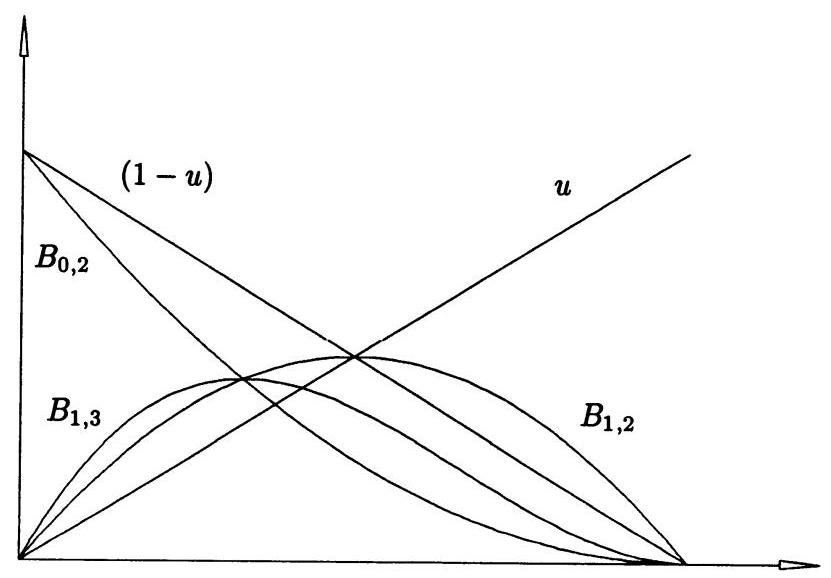
\includegraphics[max width=0.7\textwidth]{images/0193ba0d-ab19-7138-9798-cb281ce60de0_29_344_1493_831_578_0.jpg}
\end{center}
\hspace*{3em} 

图 1.14. Bernstein 多项式的递归定义， \({B}_{1,3}\left( u\right)\) 。

\begin{center}
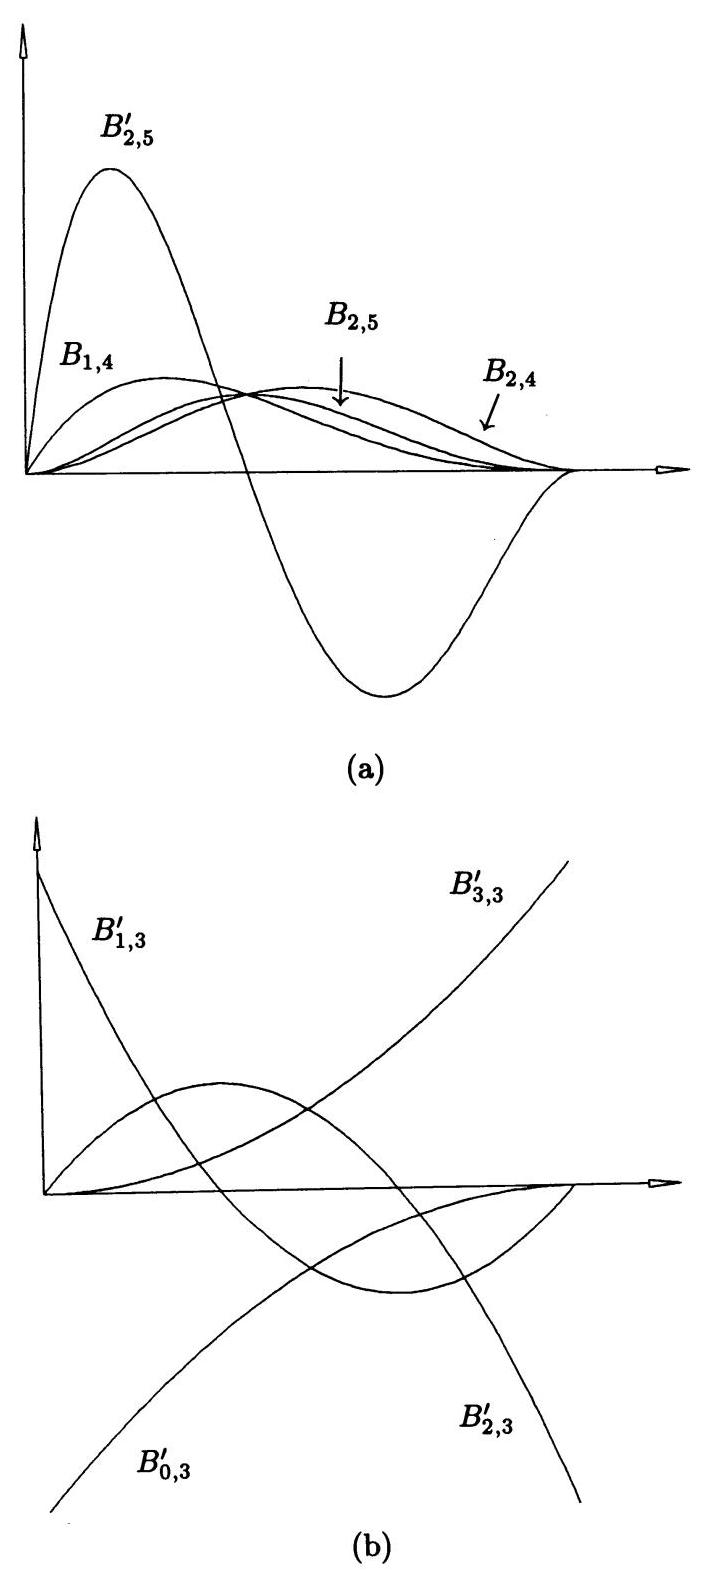
\includegraphics[max width=0.6\textwidth]{images/0193ba0d-ab19-7138-9798-cb281ce60de0_30_402_263_703_1572_0.jpg}
\end{center}
\hspace*{3em} 

图 1.15. 导数。 (a) 关于 \({B}_{1,4}\left( u\right)\) 和 \({B}_{2,4}\left( u\right)\) 的导数 \({B}_{2,5}^{\prime }\left( u\right)\) ；(b) 四个三次 Bernstein 多项式的导数， \({B}_{0,3}^{\prime }\left( u\right) ;{B}_{1,3}^{\prime }\left( u\right) ;{B}_{2,3}^{\prime }\left( u\right)\) ； \({B}_{3,3}^{\prime }\left( u\right)\) 。

性质 P1.6 产生简单的算法来计算在固定值 \(u\) 下 Bernstein 多项式的值。算法 A1.2 计算固定 \(u\) 下的值 \({B}_{i,n}\left( u\right)\) 。 \({B}_{1,3}\) 的计算如表 1.1 所示。

\HRule

ALGORITHM A1.2

\hspace*{2em} Bernstein(i, n, u, B)

\hspace*{5em} \{ /* Compute the value of a Bernstein polynomial. */

\hspace*{8em} /* Input: i, n, u */

\hspace*{8em} /* Output: B */

\hspace*{5em} for \(\left( {j = 0;j <  = n;j +  + }\right) / *\) compute the columns \(*\) /

\hspace*{7em} temp[j] = 0.0 ; /* of Table 1.1 */

\hspace*{5em} temp \(\left\lbrack  {n - i}\right\rbrack   = {1.0};\;/ *\) in a temporary array \(*\) /

\hspace*{5em} u1 = 1.0-u;

\hspace*{5em} for (k=1; k<=n; k++)

\hspace*{7em} for (j=n; j>=k; j--)

\hspace*{9em} temp[j] = u1*temp[j] + u*temp[j-1];

\hspace*{5em} B = temp[n];

\hspace*{4em} \}

\HRule

算法 A1.3 计算在固定 \(u\) 处非零的 \(n + {1n}\) 次伯恩斯坦多项式。它避免了不必要的零项计算。该算法在表 1.2 中展示了立方体的情况。

算法 A1.3

AllBernstein (n, u, B)

\begin{center}
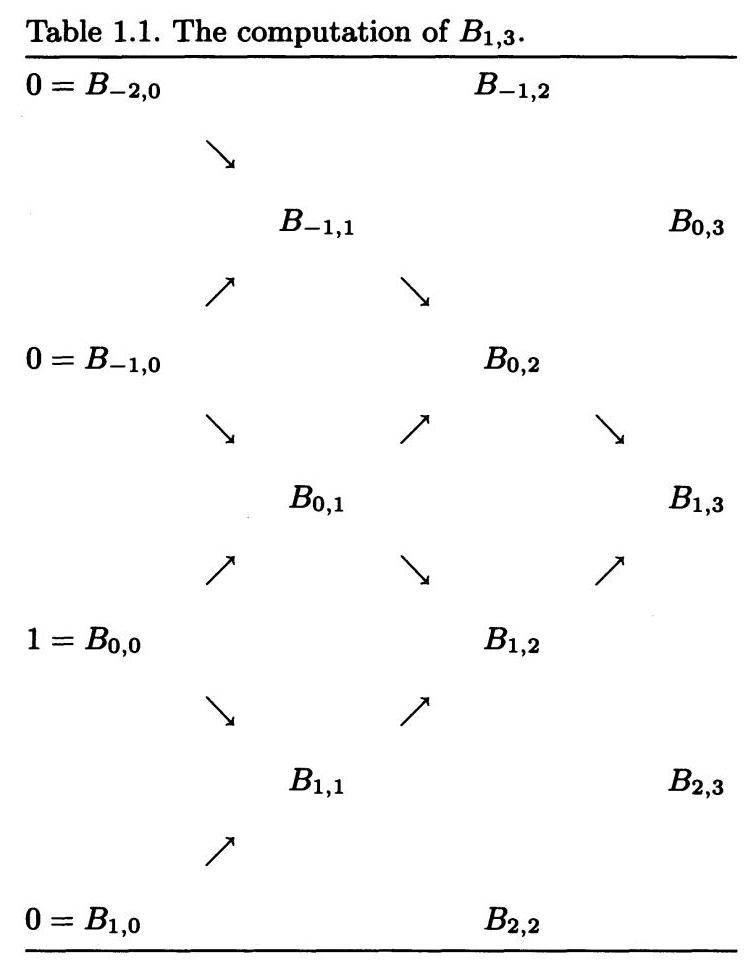
\includegraphics[max width=0.6\textwidth]{images/0193ba0d-ab19-7138-9798-cb281ce60de0_31_388_1185_748_964_0.jpg}
\end{center}
\hspace*{3em} 

\section*{贝塞尔曲线 21}

表 1.2. 所有立方伯恩斯坦的计算

\begin{center}
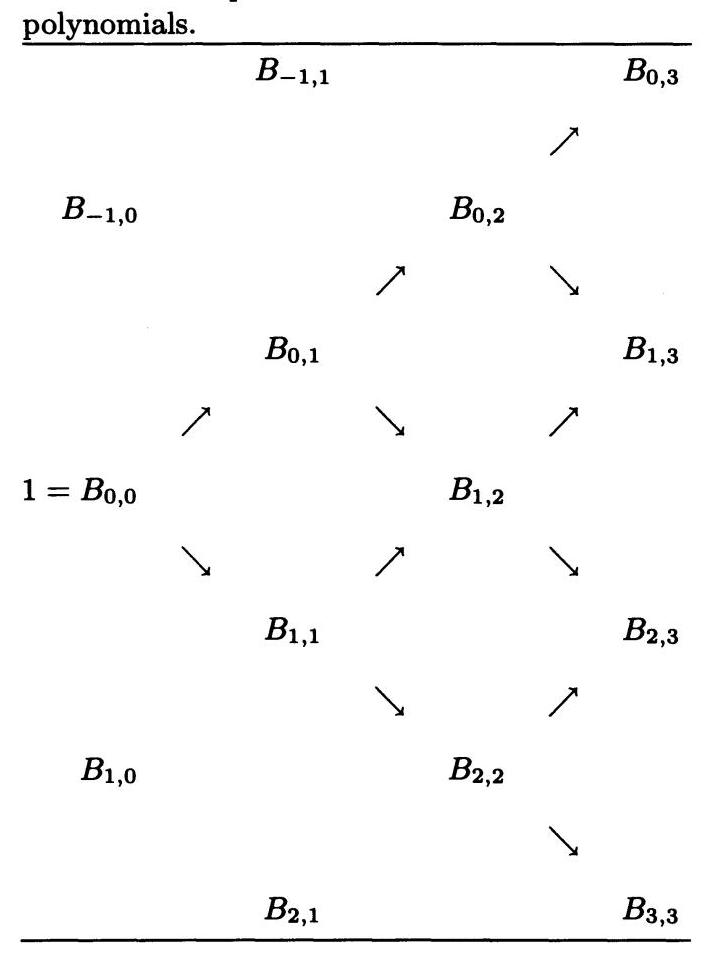
\includegraphics[max width=0.6\textwidth]{images/0193ba0d-ab19-7138-9798-cb281ce60de0_32_413_297_710_957_0.jpg}
\end{center}
\hspace*{3em} 

\HRule

\hspace*{9em} \{ /* Compute all nth-degree Bernstein polynomials. */

\hspace*{12em} /* Input: n, u */

\hspace*{12em} /* Output: B (an array, B[0],..., B[n]) */

\hspace*{8em} B[0] = 1.0;

\hspace*{8em} u1 = 1.0-u;

\hspace*{8em} for (j=1; j<=n; j++)

\hspace*{11em} \{

\hspace*{11em} saved \(= {0.0}\) ;

\hspace*{11em} for \(\left( {k = 0;k < j;k +  + }\right)\)

\hspace*{13em} \{

\hspace*{13em} temp = B[k];

\hspace*{13em} B[k] = saved+u1*temp;

\hspace*{13em} saved = u*temp;

\hspace*{13em} \}

\hspace*{11em} \(B\left\lbrack  j\right\rbrack   =\) saved;

\hspace*{11em} \}

\hspace*{8em} \}

\hspace*{2em} Algorithm A1.4 combines A1.3 and Eq. (1.7) to compute the point on an

\(n\) th-degree Bézier curve at a fixed \(u\) value.

\HRule

算法 A1.4

PointOnBezierCurve(P, n, u, C)

\{ /* 计算贝塞尔曲线上的点。 */

/* 输入: P, n, u */

/* 输出: C (一个点) */

AllBernstein \(\left( {n,u,B}\right) \;/ * B\) 是一个局部数组 \(*\) /

C = 0.0 ;

对于 \(\left( {k = 0;k <  = n;k +  + }\right) \;C = C + B\left\lbrack  k\right\rbrack   * P\left\lbrack  k\right\rbrack\) ;

\}

使用性质 P1.7，可以轻松推导出 Bézier 曲线导数的一般表达式。

\[
{\mathbf{C}}^{\prime }\left( u\right)  = \frac{d\left( {\mathop{\sum }\limits_{{i = 0}}^{n}{B}_{i,n}\left( u\right) {\mathbf{P}}_{i}}\right) }{du} = \mathop{\sum }\limits_{{i = 0}}^{n}{B}_{i,n}^{\prime }\left( u\right) {\mathbf{P}}_{i}
\]

\[
= \mathop{\sum }\limits_{{i = 0}}^{n}n\left( {{B}_{i - 1,n - 1}\left( u\right)  - {B}_{i,n - 1}\left( u\right) }\right) {\mathbf{P}}_{i}
\]

\[
= n\mathop{\sum }\limits_{{i = 0}}^{{n - 1}}{B}_{i,n - 1}\left( u\right) \left( {{\mathbf{P}}_{i + 1} - {\mathbf{P}}_{i}}\right)  \tag{1.9}
\]

从公式 (1.9) 我们可以轻松获得 Bézier 曲线的端点导数公式，例如。

\[
{\mathbf{C}}^{\prime }\left( 0\right)  = n\left( {{\mathbf{P}}_{1} - {\mathbf{P}}_{0}}\right) \;{\mathbf{C}}^{\prime \prime }\left( 0\right)  = n\left( {n - 1}\right) \left( {{\mathbf{P}}_{0} - 2{\mathbf{P}}_{1} + {\mathbf{P}}_{2}}\right)
\]

\[
{\mathbf{C}}^{\prime }\left( 1\right)  = n\left( {{\mathbf{P}}_{n} - {\mathbf{P}}_{n - 1}}\right) \;{\mathbf{C}}^{\prime \prime }\left( 1\right)  = n\left( {n - 1}\right) \left( {{\mathbf{P}}_{n} - 2{\mathbf{P}}_{n - 1} + {\mathbf{P}}_{n - 2}}\right)  \tag{1.10}
\]

从公式 (1.9) 和 (1.10) 注意到:

\begin{itemize}
\item 一个 \(n\) 次 Bézier 曲线的导数是一个 (n - 1) 次 Bézier 曲线；
\end{itemize}

\begin{itemize}
\item 在 \(u = 0\) 和 \(u = 1\) 处的端点导数表达式是对称的(当然，这是由于基函数的对称性)；
\end{itemize}

\begin{itemize}
\item 在一个端点的 \(k\) 次导数仅依赖于该端点的 \(k + 1\) 控制点(以几何上非常直观的方式)。
\end{itemize}

设 \(n = 2\) 和 \(\mathbf{C}\left( u\right)  = \mathop{\sum }\limits_{{i = 0}}^{2}{B}_{i,2}\left( u\right) {\mathbf{P}}_{i}\) 。那么

\[
\mathbf{C}\left( u\right)  = {\left( 1 - u\right) }^{2}{\mathbf{P}}_{0} + {2u}\left( {1 - u}\right) {\mathbf{P}}_{1} + {u}^{2}{\mathbf{P}}_{2}
\]

\[
= \left( {1 - u}\right) \left( \underset{\text{ linear }}{\underbrace{\left( {1 - u}\right) {\mathbf{P}}_{0} + u{\mathbf{P}}_{1}}}\right)  + u\left( \underset{\text{ linear }}{\underbrace{\left( {1 - u}\right) {\mathbf{P}}_{1} + u{\mathbf{P}}_{2}}}\right)
\]

因此， \(\mathbf{C}\left( u\right)\) 是两个一阶 Bézier 曲线的线性插值；特别地， \(\mathbf{C}\left( u\right)\) 上的任何点都是通过三次线性插值得到的。

\begin{center}
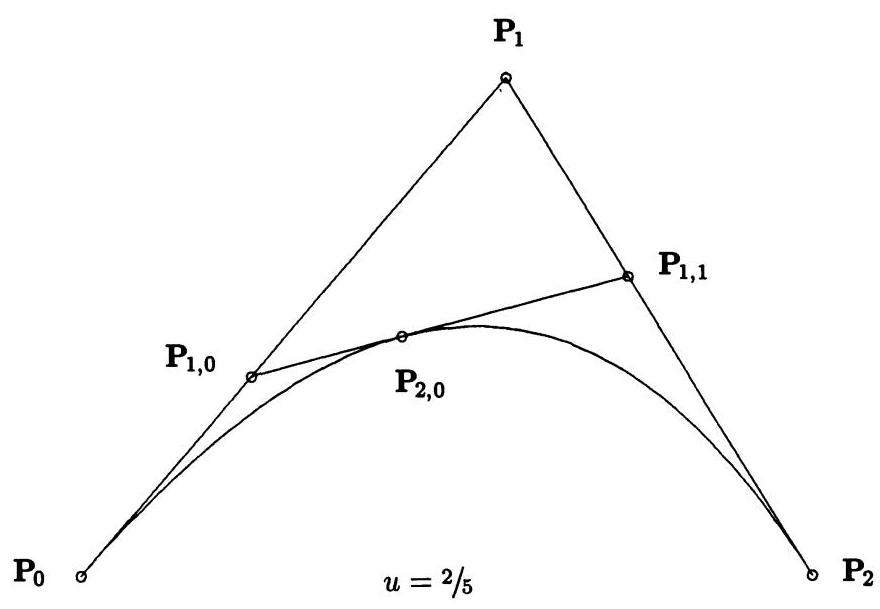
\includegraphics[max width=0.8\textwidth]{images/0193ba0d-ab19-7138-9798-cb281ce60de0_34_325_283_880_609_0.jpg}
\end{center}
\hspace*{3em} 

图 1.16. 通过在 \({u}_{0} = 2/5\) 处重复线性插值得到二次 Bézier 曲线上的一个点。

假设固定 \(u = {u}_{0}\) 并让 \({\mathbf{P}}_{1,0} = \left( {1 - {u}_{0}}\right) {\mathbf{P}}_{0} + {u}_{0}{\mathbf{P}}_{1},{\mathbf{P}}_{1,1} = (1 -\)  \(\left. {u}_{0}\right) {\mathbf{P}}_{1} + {u}_{0}{\mathbf{P}}_{2}\) 和 \({\mathbf{P}}_{2,0} = \left( {1 - {u}_{0}}\right) {\mathbf{P}}_{1,0} + {u}_{0}{\mathbf{P}}_{1,1}\) ，那么 \(\mathbf{C}\left( {u}_{0}\right)  =\)  \({\mathbf{P}}_{2,0}\) 。该情况在图 1.16 中描绘，三次情况在图 1.17 中显示。

表示一般的 \(n\) 阶 Bézier 曲线为 \({\mathbf{C}}_{n}\left( {{\mathbf{P}}_{0},\ldots ,{\mathbf{P}}_{n}}\right)\) ，我们有

\[
{\mathbf{C}}_{n}\left( {{\mathbf{P}}_{0},\ldots ,{\mathbf{P}}_{n}}\right)  = \left( {1 - u}\right) {\mathbf{C}}_{n - 1}\left( {{\mathbf{P}}_{0},\ldots ,{\mathbf{P}}_{n - 1}}\right)
\]

\[
+ u{\mathbf{C}}_{n - 1}\left( {{\mathbf{P}}_{1},\ldots ,{\mathbf{P}}_{n}}\right)  \tag{1.11}
\]

这源于基函数的递归定义(见 P1.6)。固定 \(u = {u}_{0}\) 并将 \({\mathbf{P}}_{i}\) 表示为 \({\mathbf{P}}_{0,i}\) ，方程 (1.11) 产生了计算 \(\mathbf{C}\left( {u}_{0}\right)  = {\mathbf{P}}_{n,0}\left( {u}_{0}\right)\) 在 \(n\) 阶 Bézier 曲线上的递归算法，即

\[
{\mathbf{P}}_{k,i}\left( {u}_{0}\right)  = \left( {1 - {u}_{0}}\right) {\mathbf{P}}_{k - 1,i}\left( {u}_{0}\right)  + {u}_{0}{\mathbf{P}}_{k - 1,i + 1}\left( {u}_{0}\right) \;\text{ for }\left\{  \begin{array}{l} k = 1,\ldots ,n \\  i = 0,\ldots ,n - k \end{array}\right.  \tag{1.12}
\]

\begin{center}
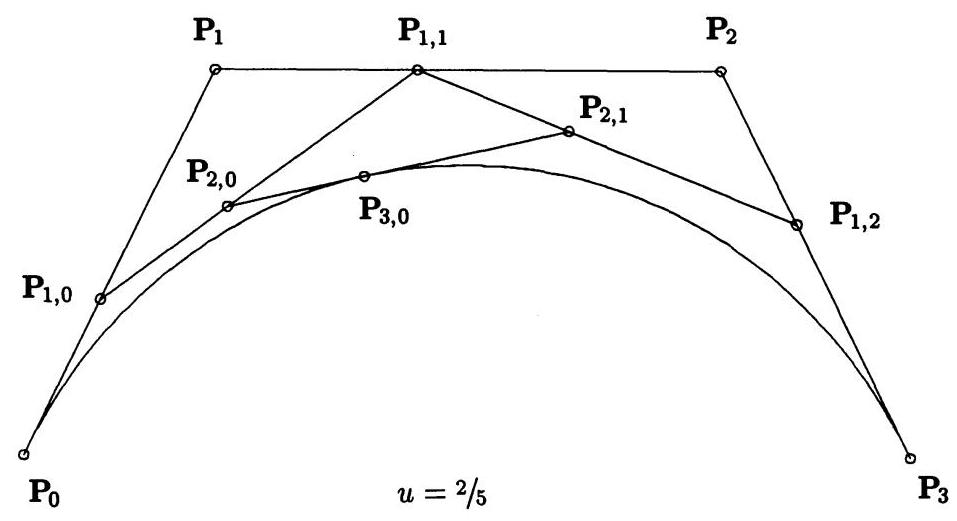
\includegraphics[max width=0.8\textwidth]{images/0193ba0d-ab19-7138-9798-cb281ce60de0_34_283_1547_957_521_0.jpg}
\end{center}
\hspace*{3em} 

图 1.17. 通过在 \({u}_{0} = 2/5\) 处重复线性插值得到的三次 Bézier 曲线上的一个点。

方程 (1.12) 被称为 deCasteljau 算法(见 [Boeh84; deCa86, 93])。它是一个切角过程(见图 1.16 和 1.17)，生成表 1.3 中所示的点的三角形表。

\HRule

ALGORITHM A1.5

\hspace*{2em} deCasteljau1(P, n, u, C)

\hspace*{4em} \{ /* Compute point on a Bézier curve */

\hspace*{7em} /* using deCasteljau */

\hspace*{7em} /* Input: P, n, u */

\hspace*{7em} /* Output: C (a point) */

\hspace*{4em} for (i=0; i<=n; i++) /* Use local array so we do not */

\hspace*{6em} \(Q\left\lbrack  i\right\rbrack   = P\left\lbrack  i\right\rbrack  ;\;/ *\) destroy control points \(* /\)

\hspace*{4em} for ( \(k = 1\) ; \(k <  = n\) ; \(k +  +\) )

\hspace*{6em} for (i = 0; i<=n-k; i++)

\hspace*{8em} \(\mathrm{Q}\left\lbrack  \mathrm{i}\right\rbrack   = \left( {{1.0} - \mathrm{u}}\right)  * \mathrm{Q}\left\lbrack  \mathrm{i}\right\rbrack   + \mathrm{u} * \mathrm{Q}\left\lbrack  {\mathrm{i} + 1}\right\rbrack  ;\)

\hspace*{4em} C = Q[0];

\hspace*{4em} \}

\HRule

我们以 Bézier 方法和幂基方法的比较结束本节。显然，Bézier 形式在两者中更具几何性。方程 (1.10) 结合凸包和变差减小特性，使得

表 1.3. 由 deCasteljau 算法生成的点。

\({\mathbf{P}}_{0}\)

\({\mathbf{P}}_{1,0}\)

\({\mathbf{P}}_{1}\)  \({\mathbf{P}}_{2,0}\)

\({\mathbf{P}}_{1,1}\)

\({\mathbf{P}}_{2}\)

\({\mathbf{P}}_{n - 1,0}\)

\(\vdots \;\vdots \;\vdots \;\cdots\)  \({\mathbf{P}}_{n,0} = \mathbf{C}\left( {u}_{0}\right)\)

\({\mathbf{P}}_{n - 1,1}\)

\({\mathbf{P}}_{n - 2}\)

\({\mathbf{P}}_{1,n - 2}\)

\({\mathbf{P}}_{n - 1}\)  \({\mathbf{P}}_{2,n - 2}\)

\({\mathbf{P}}_{1,n - 1}\)

\({\mathbf{P}}_{n}\)

Bézier 曲线更适合于交互式曲线设计。控制点为设计师提供了比幂基系数更直观的曲线形状把握。此外，deCasteljau 算法比霍纳算法更不容易受到舍入误差的影响。当考虑到 deCasteljau 算法仅仅是在曲线附近的点之间进行重复线性插值时，这一点是直观清晰的。Bézier 形式的唯一缺点是点评估效率较低(见算法 A1.1、A1.4 和 A1.5，以及本章后面的练习 1.13)。



\section{有理 Bézier 曲线}

接下来，我们介绍有理曲线和齐次坐标的概念。为了说明这些概念，我们简要介绍有理贝塞尔曲线。这些曲线是有理B样条曲线的特例，因此在后续章节中将更全面和严格地处理。

尽管多项式提供了许多优势，但存在一些重要的曲线和曲面类型无法用多项式精确表示，例如圆、椭圆、双曲线、圆柱、圆锥、球体等。作为一个例子，我们证明单位圆在 \({xy}\) 平面中，以原点为中心，无法用多项式坐标函数表示。相反，假设

\[
x\left( u\right)  = {a}_{0} + {a}_{1}u + \cdots  + {a}_{n}{u}^{n}
\]

\[
y\left( u\right)  = {b}_{0} + {b}_{1}u + \cdots  + {b}_{n}{u}^{n}
\]

然后 \({x}^{2} + {y}^{2} - 1 = 0\) 意味着

\[
0 = {\left( {a}_{0} + {a}_{1}u + \cdots  + {a}_{n}{u}^{n}\right) }^{2} + {\left( {b}_{0} + {b}_{1}u + \cdots  + {b}_{n}{u}^{n}\right) }^{2} - 1
\]

\[
= \left( {{a}_{0}^{2} + {b}_{0}^{2} - 1}\right)  + 2\left( {{a}_{0}{a}_{1} + {b}_{0}{b}_{1}}\right) u + \left( {{a}_{1}^{2} + 2{a}_{0}{a}_{2} + {b}_{1}^{2} + 2{b}_{0}{b}_{2}}\right) {u}^{2}
\]

\[
+ \cdots  + \left( {{a}_{n - 1}^{2} + 2{a}_{n - 2}{a}_{n} + {b}_{n - 1}^{2} + 2{b}_{n - 2}{b}_{n}}\right) {u}^{{2n} - 2}
\]

\[
+ 2\left( {{a}_{n}{a}_{n - 1} + {b}_{n}{b}_{n - 1}}\right) {u}^{{2n} - 1} + \left( {{a}_{n}^{2} + {b}_{n}^{2}}\right) {u}^{2n}
\]

这个方程必须对所有 \(u\) 成立，这意味着所有系数都是零。从最高次开始逐步推导，我们在 \(n\) 步骤中证明所有 \({a}_{i} = 0\) 和 \({b}_{i} = 0\) 对于 \(1 \leq  i \leq  n\) 。

步骤

1. \({a}_{n}^{2} + {b}_{n}^{2} = 0\) 意味着 \({a}_{n} = {b}_{n} = 0\) 。

2. \({a}_{n - 1}^{2} + 2{a}_{n - 2}{a}_{n} + {b}_{n - 1}^{2} + 2{b}_{n - 2}{b}_{n} = 0\) 和步骤1意味着 \({a}_{n - 1}^{2} + {b}_{n - 1}^{2} = 0\) ，这意味着 \({a}_{n - 1} = {b}_{n - 1} = 0\) 。

n. \({a}_{1}^{2} + 2{a}_{0}{a}_{2} + {b}_{1}^{2} + 2{b}_{0}{b}_{2} = 0\) 和步骤 \(n - 1\) 意味着 \({a}_{1}^{2} + {b}_{1}^{2} = 0\) ，这意味着 \({a}_{1} = {b}_{1} = 0\) 。

因此， \(x\left( u\right)  = {a}_{0}\) 和 \(y\left( u\right)  = {b}_{0}\) ，这是一个明显的矛盾。

从经典数学中已知，所有的圆锥曲线，包括圆，都可以用有理函数表示，有理函数被定义为两个多项式的比率。实际上，它们是用有理函数表示的

形式为

\[
x\left( u\right)  = \frac{X\left( u\right) }{W\left( u\right) }\;y\left( u\right)  = \frac{Y\left( u\right) }{W\left( u\right) } \tag{1.13}
\]

其中 \(X\left( u\right) ,Y\left( u\right)\) 和 \(W\left( u\right)\) 是多项式，也就是说，每个坐标函数具有相同的分母。

\section*{示例}

Ex1.8 半径为 1 的圆，中心位于原点

\[
x\left( u\right)  = \frac{1 - {u}^{2}}{1 + {u}^{2}}\;y\left( u\right)  = \frac{2u}{1 + {u}^{2}}
\]

Ex1.9 椭圆，中心位于原点； \(y\) 轴是主轴， \(x\) 轴是次轴，主半径和次半径分别为 2 和 1

\[
x\left( u\right)  = \frac{1 - {u}^{2}}{1 + {u}^{2}}\;y\left( u\right)  = \frac{4u}{1 + {u}^{2}}
\]

Ex1.10 双曲线，中心在 \(\mathbf{P} = \left( {0,4/3}\right)\) ； \(y\) 轴是横轴

\[
x\left( u\right)  = \frac{-1 + {2u}}{1 + {2u} - 2{u}^{2}}\;y\left( u\right)  = \frac{{4u}\left( {1 - u}\right) }{1 + {2u} - 2{u}^{2}}
\]

下支(顶点在 \(\mathbf{P} = \left( {0,2/3}\right)\) )的轨迹为

\[
u \in  \left( {\frac{1 - \sqrt{3}}{2},\frac{1 + \sqrt{3}}{2}}\right)
\]

Ex1.11 抛物线，顶点在原点； \(y\) 轴是对称轴

\[
x\left( u\right)  = u\;y\left( u\right)  = {u}^{2}
\]

注意，抛物线不需要有理函数。读者应绘制这些函数。对于圆的方程，很容易看出，对于任何 \(u,\left( {x\left( u\right) ,y\left( u\right) }\right)\) 都位于以原点为中心的单位圆上

\[
{\left( x\left( u\right) \right) }^{2} + {\left( y\left( u\right) \right) }^{2} = {\left( \frac{1 - {u}^{2}}{1 + {u}^{2}}\right) }^{2} + {\left( \frac{2u}{1 + {u}^{2}}\right) }^{2}
\]

\[
= \frac{1 - 2{u}^{2} + {u}^{4} + 4{u}^{2}}{{\left( 1 + {u}^{2}\right) }^{2}} = \frac{{\left( 1 + {u}^{2}\right) }^{2}}{{\left( 1 + {u}^{2}\right) }^{2}} = 1
\]

定义一个 \(n\) 次有理贝塞尔曲线(见 [Forr68; Pieg86; Fari83,89])

\[
\mathbf{C}\left( u\right)  = \frac{\mathop{\sum }\limits_{{i = 0}}^{n}{B}_{i,n}\left( u\right) {w}_{i}{\mathbf{P}}_{i}}{\mathop{\sum }\limits_{{i = 0}}^{n}{B}_{i,n}\left( u\right) {w}_{i}}\;0 \leq  u \leq  1 \tag{1.14}
\]

\({\mathbf{P}}_{i} = \left( {{x}_{i},{y}_{i},{z}_{i}}\right)\) 和 \({B}_{i,n}\left( u\right)\) 与之前相同； \({w}_{i}\) 是标量，称为权重。因此， \(W\left( u\right)  = \mathop{\sum }\limits_{{i = 0}}^{n}{B}_{i,n}\left( u\right) {w}_{i}\) 是公共分母函数。除非另有明确说明，否则我们假设对于所有 \(i\) 有 \({w}_{i} > 0\) 。这确保了对于所有 \(u \in  \left\lbrack  {0,1}\right\rbrack\) 有 \(W\left( u\right)  > 0\) 。我们写

\[
\mathbf{C}\left( u\right)  = \mathop{\sum }\limits_{{i = 0}}^{n}{R}_{i,n}\left( u\right) {\mathbf{P}}_{i}\;0 \leq  u \leq  1 \tag{1.15}
\]

其中

\[
{R}_{i,n}\left( u\right)  = \frac{{B}_{i,n}\left( u\right) {w}_{i}}{\mathop{\sum }\limits_{{j = 0}}^{n}{B}_{j,n}\left( u\right) {w}_{j}}
\]

\({R}_{i,n}\left( u\right)\) 是该曲线形式的有理基函数。图 1.18a 显示了三次基函数的一个示例，图 1.18b 显示了相应的三次有理 Bézier 曲线。

\({R}_{i,n}\left( u\right)\) 具有可以很容易从方程 (1.15) 及相应的 \({B}_{i,n}\left( u\right)\) 的性质推导出的特性:

P1.8 非负性:对所有 \(i,n\) 和 \(0 \leq  u \leq  1\) ，都有 \({R}_{i,n}\left( u\right)  \geq  0\) ；

P1.9 统一划分:对所有 \(0 \leq  u \leq  1\) ，都有 \(\mathop{\sum }\limits_{{i = 0}}^{n}{R}_{i,n}\left( u\right)  = 1\) ；

P1. \({10}{R}_{0,n}\left( 0\right)  = {R}_{n,n}\left( 1\right)  = 1\) ;

P1.11 \({R}_{i,n}\left( u\right)\) 在区间 \(\left\lbrack  {0,1}\right\rbrack\) 上恰好达到一个最大值；

P1.12 如果对所有 \(i\) 都有 \({w}_{i} = 1\) ，那么对所有 \(i\) 都有 \({R}_{i,n}\left( u\right)  = {B}_{i,n}\left( u\right)\) ；即， \({B}_{i,n}\left( u\right)\) 是 \({R}_{i,n}\left( u\right)\) 的一个特例。

这些结果得出了有理 Bézier 曲线的以下几何特性:

P1.13 凸包性质:曲线包含在其定义控制点( \({\mathbf{P}}_{i}\) )的凸包内；

P1.14 变换不变性:通过对控制点应用旋转、平移和缩放来对曲线进行变换；

P1.15 变差减小性质:与多项式 Bézier 曲线相同(见前一节)；

P1.16 端点插值: \(\mathbf{C}\left( 0\right)  = {\mathbf{P}}_{0}\) 和 \(\mathbf{C}\left( 1\right)  = {\mathbf{P}}_{n}\) ；

P1.17 在 \(u = 0\left( {u = 1}\right)\) 处的 \(k\) 阶导数依赖于第一个(最后一个) \(k + 1\) 控制点和权重；特别地， \({\mathbf{C}}^{\prime }\left( 0\right)\) 和 \({\mathbf{C}}^{\prime }\left( 1\right)\) 分别与 \({\mathbf{P}}_{1} - {\mathbf{P}}_{0}\) 和 \({\mathbf{P}}_{n} - {\mathbf{P}}_{n - 1}\) 平行；

P1.18 多项式贝塞尔曲线是有理贝塞尔曲线的一个特例。

\begin{center}
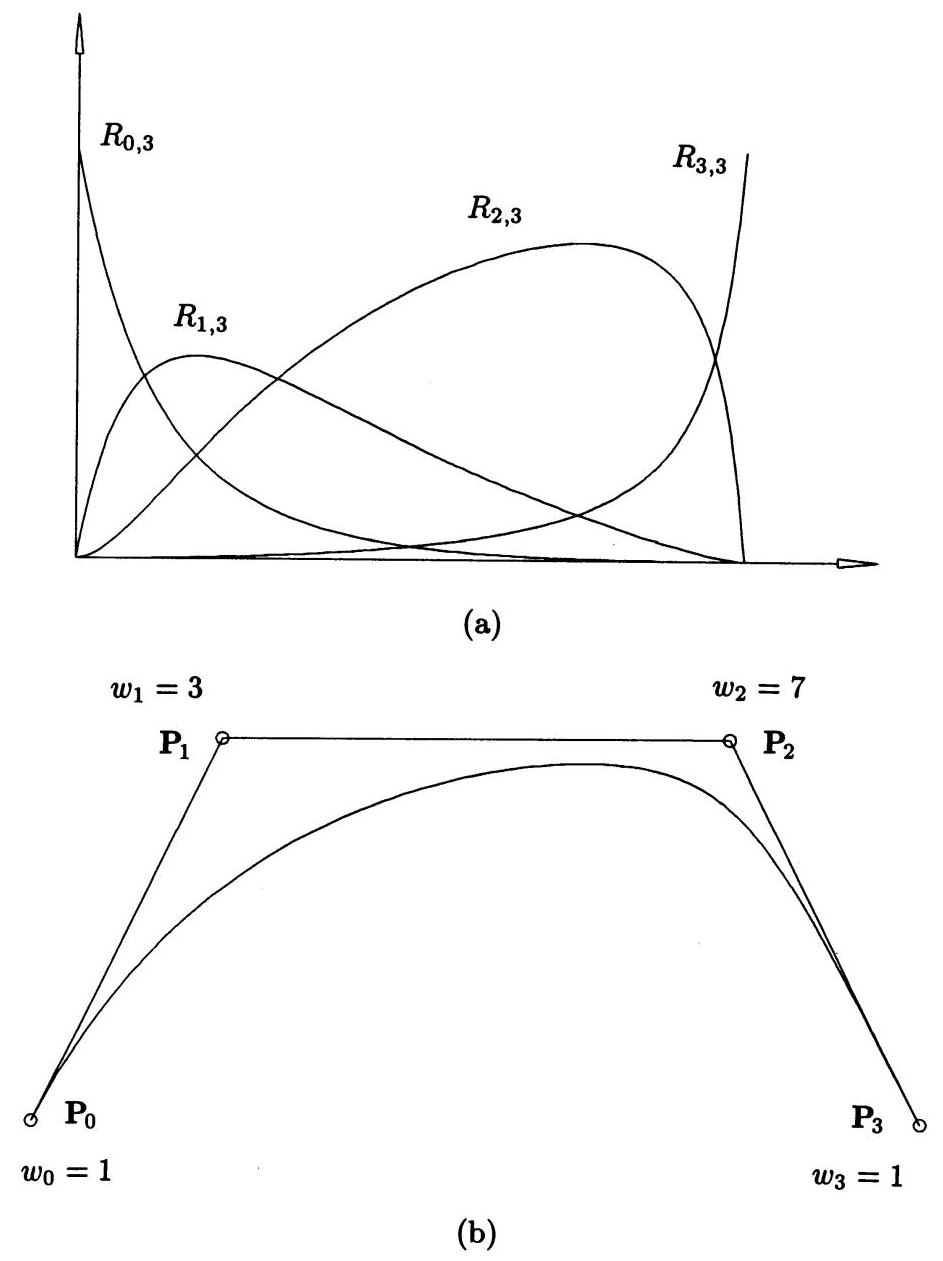
\includegraphics[max width=0.8\textwidth]{images/0193ba0d-ab19-7138-9798-cb281ce60de0_39_302_260_943_1261_0.jpg}
\end{center}
\hspace*{3em} 

图 1.18. 有理三次曲线。 (a) 基函数；(b) 贝塞尔曲线。

\section*{示例}

Ex1.12 让我们考虑有理贝塞尔圆弧。

\[
\mathbf{C}\left( u\right)  = \left( {x\left( u\right) ,y\left( u\right) }\right)  = \left( {\frac{1 - {u}^{2}}{1 + {u}^{2}},\frac{2u}{1 + {u}^{2}}}\right) \;0 \leq  u \leq  1
\]

表示单位圆的一个象限，如图 1.19a 所示。我们现在推导这个圆弧的二次有理贝塞尔表示。显然，从 P1.16 和 P1.17 可得 \({\mathbf{P}}_{0} = \left( {1,0}\right) ,{\mathbf{P}}_{1} = \left( {1,1}\right)\) 和 \({\mathbf{P}}_{2} = \left( {0,1}\right)\) 。对于权重，我们有

\[
W\left( u\right)  = 1 + {u}^{2} = \mathop{\sum }\limits_{{i = 0}}^{2}{B}_{i,2}\left( u\right) {w}_{i} = {\left( 1 - u\right) }^{2}{w}_{0} + {2u}\left( {1 - u}\right) {w}_{1} + {u}^{2}{w}_{2}
\]

\begin{center}
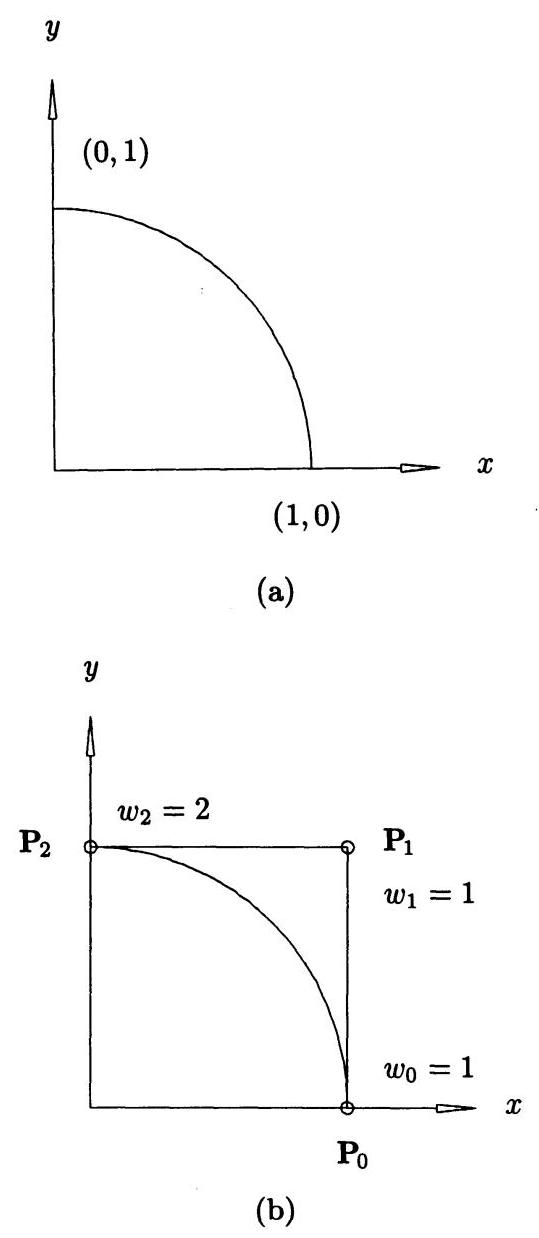
\includegraphics[max width=0.4\textwidth]{images/0193ba0d-ab19-7138-9798-cb281ce60de0_40_499_257_539_1238_0.jpg}
\end{center}
\hspace*{3em} 

图 1.19. 单位圆的表示。 (a) 一个象限的 \(x\left( u\right)  = \left( {1 - {u}^{2}}\right) /\left( {1 + {u}^{2}}\right)\) 和 \(y\left( u\right)  = \left( {2u}\right) /\left( {1 + {u}^{2}}\right)\) ；(b) 与图 \({1.19}\mathrm{a}\left( {{w}_{0} = 1,{w}_{1} = 1,{w}_{2} = 2}\right)\) 对应的贝塞尔表示。

代入 \(u = 0\) 得到 \({w}_{0} = 1\) ，代入 \(u = 1\) 得到 \({w}_{2} = 2\) 。最后，代入 \(u = 1/2\) 得到 \(5/4 = 1/4{w}_{0} + 1/2{w}_{1} + 1/4{w}_{2}\) ，并使用 \({w}_{0} = 1\) 和 \({w}_{2} = 2\) 得到 \({w}_{1} = 1\) (见图 1.19b)。

具有形式为 Eq. (1.13)(一个共同分母)的坐标函数的有理曲线具有优雅的几何解释，这种解释能够实现高效处理和紧凑的数据存储。其思想是使用齐次坐标将有理曲线表示为 \(n\) 维空间中的多项式曲线(见 [Robe65; Ries81; Patt85])。我们从三维欧几里得空间中的一个点 \(\mathbf{P} = \left( {x,y,z}\right)\) 开始。然后 \(\mathbf{P}\) 在四维空间 \(w \neq  0\) 中写作 \({\mathbf{P}}^{w} = \left( {{wx},{wy},{wz},w}\right)  = \left( {X,Y,Z,W}\right)\) 。现在

\(\mathbf{P}\) 是通过将所有坐标除以第四个坐标 \(W\) 得到的，即通过将 \({\mathbf{P}}^{w}\) 从原点映射到超平面 \(W = 1\) (见图 1.20 的二维情况， \(\mathbf{P} = \left( {x,y}\right) )\) )。该映射，记作 \(H\) ，是一个以原点为中心的透视映射。

\[
\mathbf{P} = H\left\{  {\mathbf{P}}^{w}\right\}   = H\{ \left( {X,Y,Z,W}\right) \}  = \left\{  \begin{array}{ll} \left( {\frac{X}{W},\frac{Y}{W},\frac{Z}{W}}\right) & \text{ if }W \neq  0 \\  \text{ direction }\left( {X,Y,Z}\right) & \text{ if }W = 0 \end{array}\right.  \tag{1.16}
\]

注意，对于任意的 \(x,y,z,{w}_{1},{w}_{2}\) ，其中 \({w}_{1} \neq  {w}_{2}\)

\[
H\left\{  {\mathbf{P}}^{{w}_{1}}\right\}   = H\left\{  \left( {{w}_{1}x,{w}_{1}y,{w}_{1}z,{w}_{1}}\right) \right\}   = \left( {x,y,z}\right)
\]

\[
= H\left\{  \left( {{w}_{2}x,{w}_{2}y,{w}_{2}z,{w}_{2}}\right) \right\}   = H\left\{  {\mathbf{P}}^{{w}_{2}}\right\}
\]

现在，对于给定的一组控制点 \(\left\{  {\mathbf{P}}_{i}\right\}\) 和权重 \(\left\{  {w}_{i}\right\}\) ，构造加权控制点 \({\mathbf{P}}_{i}^{w} = \left( {{w}_{i}{x}_{i},{w}_{i}{y}_{i},{w}_{i}{z}_{i},{w}_{i}}\right)\) 。然后在四维空间中定义非有理(多项式)Bézier 曲线。

\[
{\mathbf{C}}^{w}\left( u\right)  = \mathop{\sum }\limits_{{i = 0}}^{n}{B}_{i,n}\left( u\right) {\mathbf{P}}_{i}^{w} \tag{1.17}
\]

\begin{center}
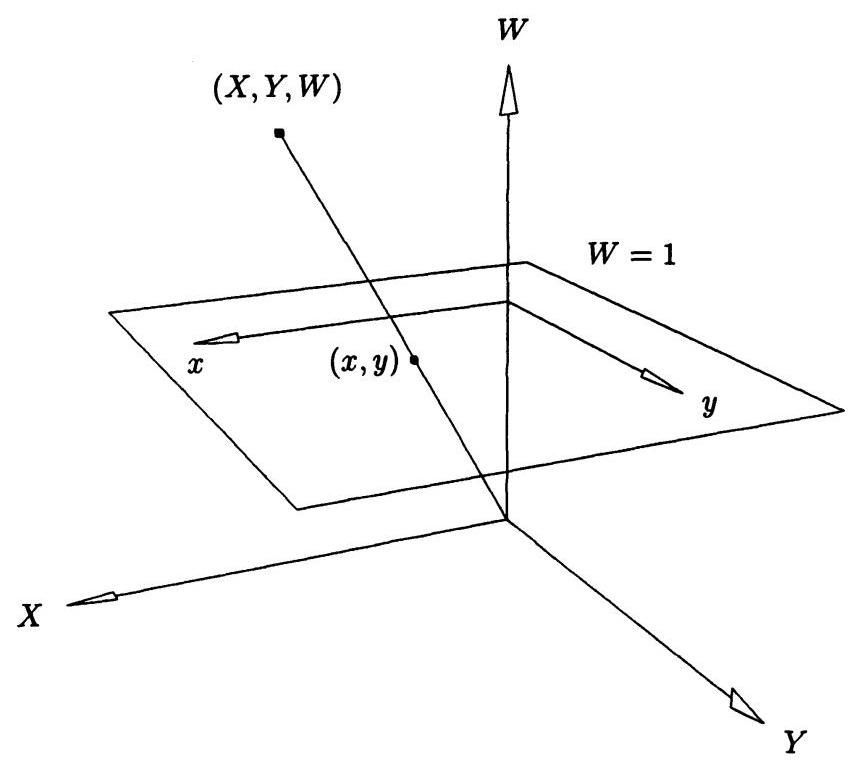
\includegraphics[max width=0.7\textwidth]{images/0193ba0d-ab19-7138-9798-cb281ce60de0_41_336_1298_858_767_0.jpg}
\end{center}
\hspace*{3em} 

图 1.20. 齐次形式下的欧几里得点的表示。

然后，将透视映射 \(H\) 应用于 \({\mathbf{C}}^{w}\left( u\right)\) ，得到 Eq. (1.14) 的相应有理 Bézier 曲线(见图 1.21)，即写出 Eq. (1.17) 的坐标函数，我们得到

\[
X\left( u\right)  = \mathop{\sum }\limits_{{i = 0}}^{n}{B}_{i,n}\left( u\right) {w}_{i}{x}_{i}\;Y\left( u\right)  = \mathop{\sum }\limits_{{i = 0}}^{n}{B}_{i,n}\left( u\right) {w}_{i}{y}_{i}
\]

\[
Z\left( u\right)  = \mathop{\sum }\limits_{{i = 0}}^{n}{B}_{i,n}\left( u\right) {w}_{i}{z}_{i}\;W\left( u\right)  = \mathop{\sum }\limits_{{i = 0}}^{n}{B}_{i,n}\left( u\right) {w}_{i}
\]

在三维空间中定位曲线得到

\[
x\left( u\right)  = \frac{X\left( u\right) }{W\left( u\right) } = \frac{\mathop{\sum }\limits_{{i = 0}}^{n}{B}_{i,n}\left( u\right) {w}_{i}{x}_{i}}{\mathop{\sum }\limits_{{i = 0}}^{n}{B}_{i,n}\left( u\right) {w}_{i}}
\]

\[
y\left( u\right)  = \frac{Y\left( u\right) }{W\left( u\right) } = \frac{\mathop{\sum }\limits_{{i = 0}}^{n}{B}_{i,n}\left( u\right) {w}_{i}{y}_{i}}{\mathop{\sum }\limits_{{i = 0}}^{n}{B}_{i,n}\left( u\right) {w}_{i}}
\]

\[
z\left( u\right)  = \frac{Z\left( u\right) }{W\left( u\right) } = \frac{\mathop{\sum }\limits_{{i = 0}}^{n}{B}_{i,n}\left( u\right) {w}_{i}{z}_{i}}{\mathop{\sum }\limits_{{i = 0}}^{n}{B}_{i,n}\left( u\right) {w}_{i}}
\]

使用向量表示法，我们得到

\[
\mathbf{C}\left( u\right)  = \left( {x\left( u\right) ,y\left( u\right) ,z\left( u\right) }\right)  = \frac{\mathop{\sum }\limits_{{i = 0}}^{n}{B}_{i,n}\left( u\right) {w}_{i}\left( {{x}_{i},{y}_{i},{z}_{i}}\right) }{\mathop{\sum }\limits_{{i = 0}}^{n}{B}_{i,n}\left( u\right) {w}_{i}}
\]

\[
= \frac{\mathop{\sum }\limits_{{i = 0}}^{n}{B}_{i,n}\left( u\right) {w}_{i}{\mathbf{P}}_{i}}{\mathop{\sum }\limits_{{i = 0}}^{n}{B}_{i,n}\left( u\right) {w}_{i}} \tag{1.18}
\]

\begin{center}
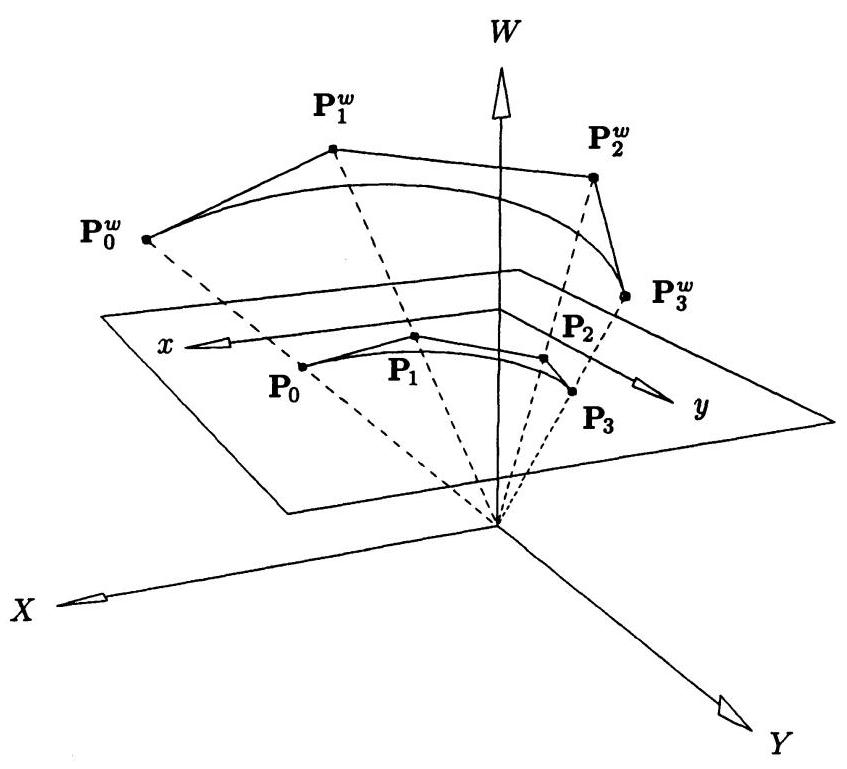
\includegraphics[max width=0.7\textwidth]{images/0193ba0d-ab19-7138-9798-cb281ce60de0_43_347_255_847_769_0.jpg}
\end{center}
\hspace*{3em} 

图 1.21. 有理 Bézier 曲线的几何构造。

本书中的算法主要使用由方程 (1.17) 给出的形式，以及有理 B 样条曲线的类似形式。因此，无理形式在四维空间中处理，结果通过映射 \(H\) 定位于三维空间中。我们可以交替地将 \({\mathbf{C}}^{w}\left( u\right)\) 或 \(\mathbf{C}\left( u\right)\) 称为有理 Bézier(或 B 样条)曲线，尽管严格来说， \({\mathbf{C}}^{w}\left( u\right)\) 不是一条有理曲线。

\section*{示例}

示例 1.13 让我们回到图 1.19b 中的圆弧。我们有 \({\mathbf{P}}_{0} = \left( {1,0}\right)\) 、 \({\mathbf{P}}_{1} = \left( {1,1}\right) ,{\mathbf{P}}_{2} = \left( {0,1}\right)\) 和 \({w}_{0} = 1,{w}_{1} = 1,{w}_{2} = 2\) 。因此，对于方程 (1.17)，三维控制点为 \(\;{\textbf{P}}_{0}^{w} = \left( {1,0,1}\right) ,\;{\textbf{P}}_{1}^{w} =\) (1,1,1) 和 \({\mathbf{P}}_{2}^{w} = \left( {0,2,2}\right)\) 。然后 \({\mathbf{C}}^{w}\left( u\right)  = {\left( 1 - u\right) }^{2}{\mathbf{P}}_{0}^{w} + {2u}\left( {1 - u}\right) {\mathbf{P}}_{1}^{w} +\)  \({u}^{2}{\mathbf{P}}_{2}^{w}\) 是一条抛物线弧(无理)，它在 \(W = 1\) 平面上投影为一条圆弧(见图 1.22)。

设 \({u}_{0}\) 为固定值。由于 \({\mathbf{C}}^{w}\left( u\right)\) 是一条多项式 Bézier 曲线，我们使用 deCasteljau 算法计算 \({\mathbf{C}}^{w}\left( {u}_{0}\right)\) ；随后，得到 \(\mathbf{C}\left( {u}_{0}\right)  =\)  \(H\left\{  {{\mathbf{C}}^{w}\left( {u}_{0}\right) }\right\}\) 。因此，我们将方程 (1.12) 应用于 \({\mathbf{P}}_{i}^{w}\) 。

\[
{\mathbf{P}}_{k,i}^{w}\left( {u}_{0}\right)  = \left( {1 - {u}_{0}}\right) {\mathbf{P}}_{k - 1,i}^{w} + {u}_{0}{\mathbf{P}}_{k - 1,i + 1}^{w}\text{ for }\left\{  \begin{array}{l} k = 1,\ldots ,n \\  i = 0,\ldots ,n - k \end{array}\right.
\]

(1.19)

\begin{center}
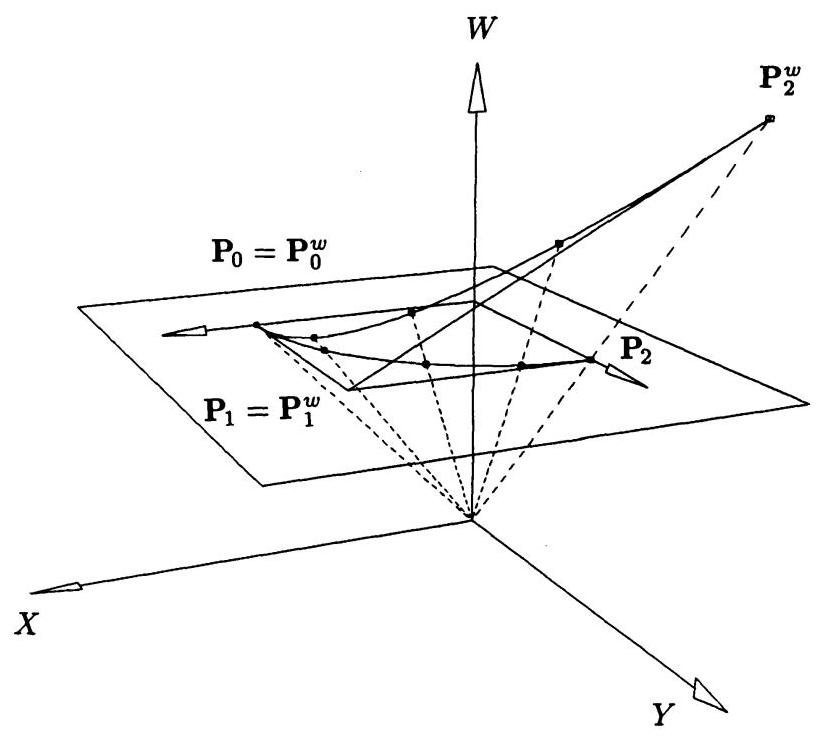
\includegraphics[max width=0.7\textwidth]{images/0193ba0d-ab19-7138-9798-cb281ce60de0_44_358_255_823_737_0.jpg}
\end{center}
\hspace*{3em} 

图 1.22. 圆弧的齐次表示。

示例 1.14 让我们应用方程 (1.19) 来计算示例 1.13 中有理 Bézier 圆弧在 \(u = 1/2\) 处的点。该弧由 \({\mathbf{C}}^{w}\left( u\right)  =\)  \({\left( 1 - u\right) }^{2}{\mathbf{P}}_{0}^{w} + {2u}\left( {1 - u}\right) {\mathbf{P}}_{1}^{w} + {u}^{2}{\mathbf{P}}_{2}^{w}\) 给出，其中 \({\mathbf{P}}_{0}^{w} = \left( {1,0,1}\right) ,{\mathbf{P}}_{1}^{w} =\)  \(\left( {1,1,1}\right) ,{\mathbf{P}}_{2}^{w} = \left( {0,2,2}\right)\) 。生成的点的三角形集合如表 1.4 所示。然后 \(\mathbf{C}\left( {1/2}\right)  = H\left\{  {{\mathbf{C}}^{w}\left( {1/2}\right) }\right\}   = H\left\{  \left( {3/4,1,5/4}\right) \right\}   = \left( {3/5,4/5}\right)\) 。

现在让我们使用我们开发的其他表示法来计算该点。设

\[
\mathbf{C}\left( u\right)  = \left( {\frac{\left( 1 - {u}^{2}\right) }{\left( 1 + {u}^{2}\right) },\frac{\left( 2u\right) }{\left( 1 + {u}^{2}\right) }}\right)
\]

表 1.4. 在圆弧上生成点 \({\mathbf{C}}^{w}\left( {1/2}\right)\) 。

\HRule

(1,0,1)

\hspace*{1em} \(\left( {1,\frac{1}{2},1}\right)\)

\(\left( {1,1,1}\right) \;\left( {\frac{3}{4},1,\frac{5}{4}}\right)  = {\mathbf{C}}^{w}\left( \frac{1}{2}\right)\)

\hspace*{1em} \(\left( {\frac{1}{2},\frac{3}{2},\frac{3}{2}}\right)\)

(0,2,2)

\HRule

\section*{34 曲线与表面基础}

然后

\[
\mathbf{C}\left( \frac{1}{2}\right)  = \left( {\frac{1 - {\left( \frac{1}{2}\right) }^{2}}{1 + {\left( \frac{1}{2}\right) }^{2}},\frac{2\left( \frac{1}{2}\right) }{1 + {\left( \frac{1}{2}\right) }^{2}}}\right)  = \left( {\frac{3}{5},\frac{4}{5}}\right)
\]

使用公式 (1.17)

\[
{\mathbf{C}}^{w}\left( \frac{1}{2}\right)  = \mathop{\sum }\limits_{{i = 0}}^{2}{B}_{i,2}\left( \frac{1}{2}\right) {\mathbf{P}}_{i}^{w} =
\]

\[
= {\left( 1 - \left( \frac{1}{2}\right) \right) }^{2}\left( {1,0,1}\right)  + 2\left( \frac{1}{2}\right) \left( {1 - \left( \frac{1}{2}\right) }\right) \left( {1,1,1}\right)
\]

\[
+ {\left( \frac{1}{2}\right) }^{2}\left( {0,2,2}\right)
\]

\[
= \frac{1}{4}\left( {1,0,1}\right)  + \frac{1}{2}\left( {1,1,1}\right)  + \frac{1}{4}\left( {0,2,2}\right)  = \left( {\frac{3}{4},1,\frac{5}{4}}\right)
\]

投影得到 \(\left( {3/5,4/5}\right)\) 。公式 (1.18) 和 (1.15) 得到相同的结果。

最后，我们注意到 \(\mathbf{C}\left( {1/2}\right)  = \left( {3/5,4/5}\right)\) 不是第一象限圆弧的中点；即，参数化不是均匀的(见第 1.1 节)。点 \(\left( {3/5,4/5}\right)\) 离起始点的弧长超过一半。这在直观上是正确的，因为通过对 \(\mathbf{C}\left( u\right)\) 进行微分，可以看出起始速度是结束速度的两倍。



\section{张量积曲面}

曲线 \(\mathbf{C}\left( u\right)\) 是一个单参数的向量值函数。它是将一段直线段映射(变形)到欧几里得三维空间中的一种方式。表面是一个双参数的向量值函数 \(u\) 和 \(v\) ，表示将 \({uv}\) 平面上的一个区域 \(\mathcal{R}\) 映射到欧几里得三维空间中的一种方式。因此，它具有形式 \(\mathbf{S}\left( {u,v}\right)  = \left( {x\left( {u,v}\right) ,y\left( {u,v}\right) ,z\left( {u,v}\right) }\right) ,\left( {u,v}\right)  \in  \mathcal{R}\) 。表示表面的方法有很多种(见 [Hosc93; Pieg89a, 93] 及 [Pieg89a] 中引用的众多参考文献)。它们在使用的坐标函数和区域类型 \(\mathcal{R}\) 上有所不同。可能最简单的方法，也是几何建模应用中最广泛使用的方法，是张量积方案。这是我们在本书其余部分中使用的方法。

张量积方法基本上是一种双向曲线方案。它使用基函数和几何系数。基函数是 \(u\) 和 \(v\) 的双变量函数，构造为单变量基函数的乘积。

几何系数在一个双向的 \(n \times  m\) 网中(拓扑上)排列。因此，张量积曲面具有以下形式

\[
\mathbf{S}\left( {u,v}\right)  = \left( {x\left( {u,v}\right) ,y\left( {u,v}\right) ,z\left( {u,v}\right) }\right)  = \mathop{\sum }\limits_{{i = 0}}^{n}\mathop{\sum }\limits_{{j = 0}}^{m}{f}_{i}\left( u\right) {g}_{j}\left( v\right) {\mathbf{b}}_{i,j} \tag{1.20}
\]

其中

\[
\left\{  \begin{array}{l} {\mathbf{b}}_{i,j} = \left( {{x}_{i,j},{y}_{i,j},{z}_{i,j}}\right) \\  0 \leq  u,v \leq  1 \end{array}\right.
\]

注意，这个映射的 (u, v) 域是一个正方形(一般来说是一个矩形)。还要注意 \(\mathbf{S}\left( {u,v}\right)\) 具有矩阵形式

\[
\mathbf{S}\left( {u,v}\right)  = {\left\lbrack  {f}_{i}\left( u\right) \right\rbrack  }^{T}\left\lbrack  {\mathbf{b}}_{i,j}\right\rbrack  \left\lbrack  {{g}_{j}\left( v\right) }\right\rbrack
\]

其中 \({\left\lbrack  {f}_{i}\left( u\right) \right\rbrack  }^{T}\) 是一个 \(\left( 1\right)  \times  \left( {n + 1}\right)\) 行向量， \(\left\lbrack  {{g}_{j}\left( v\right) }\right\rbrack\) 是一个 \(\left( {m + 1}\right)  \times  \left( 1\right)\) 列向量，而 \(\left\lbrack  {\mathbf{b}}_{i,j}\right\rbrack\) 是一个三维点的 \(\left( {n + 1}\right)  \times  \left( {m + 1}\right)\) 矩阵。

作为一个例子，我们考虑幂基曲面

\[
\mathbf{S}\left( {u,v}\right)  = \mathop{\sum }\limits_{{i = 0}}^{n}\mathop{\sum }\limits_{{j = 0}}^{m}{\mathbf{a}}_{i,j}{u}^{i}{v}^{j} = {\left\lbrack  {u}^{i}\right\rbrack  }^{T}\left\lbrack  {\mathbf{a}}_{i,j}\right\rbrack  \left\lbrack  {v}^{j}\right\rbrack  \;\left\{  \begin{array}{l} {\mathbf{a}}_{i,j} = \left( {{x}_{i,j},{y}_{i,j},{z}_{i,j}}\right) \\  0 \leq  u,v \leq  1 \end{array}\right.  \tag{1.21}
\]

我们有 \({f}_{i}\left( u\right)  = {u}^{i}\) 和 \({g}_{j}\left( v\right)  = {v}^{j}\) ，基函数是乘积 \(\left\{  {{u}^{i}{v}^{j}}\right\}\) 。如果我们固定 \(u = {u}_{0}\) ，那么

\[
{\mathbf{C}}_{{u}_{0}}\left( v\right)  = \mathbf{S}\left( {{u}_{0},v}\right)  = \mathop{\sum }\limits_{{j = 0}}^{m}\left( {\mathop{\sum }\limits_{{i = 0}}^{n}{\mathbf{a}}_{i,j}{u}_{0}^{i}}\right) {v}^{j} = \mathop{\sum }\limits_{{j = 0}}^{m}{\mathbf{b}}_{j}\left( {u}_{0}\right) {v}^{j} \tag{1.22}
\]

其中

\[
{\mathbf{b}}_{j}\left( {u}_{0}\right)  = \mathop{\sum }\limits_{{i = 0}}^{n}{\mathbf{a}}_{i,j}{u}_{0}^{i}
\]

是一个位于曲面 \(\mathbf{S}\left( {u,v}\right)\) 上的幂基曲线。 \({\mathbf{C}}_{{v}_{0}}\left( u\right)\) 是一个位于 \(\mathbf{S}\left( {u,v}\right)\) 上的幂基曲线；曲线 \({\mathbf{C}}_{{u}_{0}}\left( v\right)\) 和 \({\mathbf{C}}_{{v}_{0}}\left( u\right)\) 在曲面点 \(\mathbf{S}\left( {{u}_{0},{v}_{0}}\right)\) 处相交。这些曲线称为等参数曲线(或等曲线)。 \({\mathbf{C}}_{{u}_{0}}\left( v\right)\) 被称为 \(v\) 曲线， \({\mathbf{C}}_{{v}_{0}}\left( u\right)\) 是 \(u\) 曲线(见图 1.23)。

方程 (1.21) 可以写成

\[
\mathbf{S}\left( {u,v}\right)  = \left\{  \underset{{\mathbf{b}}_{0}}{\underbrace{{\mathbf{a}}_{0,0} + {\mathbf{a}}_{0,1}v + {\mathbf{a}}_{0,2}{v}^{2} + \cdots  + {\mathbf{a}}_{0,m}{v}^{m}}}\right\}
\]

\[
+ u\left\{  \underset{{\mathbf{b}}_{1}}{\underbrace{{\mathbf{a}}_{1,0} + {\mathbf{a}}_{1,1}v + {\mathbf{a}}_{1,2}{v}^{2} + \cdots  + {\mathbf{a}}_{1,m}{v}^{m}}}\right\}
\]

\[
+ {u}^{2}\left\{  \underset{{\mathbf{b}}_{2}}{\underbrace{{\mathbf{a}}_{2,0} + {\mathbf{a}}_{2,1}v + {\mathbf{a}}_{2,2}{v}^{2} + \cdots  + {\mathbf{a}}_{2,m}{v}^{m}}}\right\}
\]

\[
\vdots
\]

\[
+ {u}^{n}\left\{  \underset{{\mathbf{b}}_{n}}{\underbrace{{\mathbf{a}}_{n,0} + {\mathbf{a}}_{n,1}v + {\mathbf{a}}_{n,2}{v}^{2} + \cdots  + {\mathbf{a}}_{n,m}{v}^{m}}}\right\}
\]

\[
= {\mathbf{b}}_{0} + {\mathbf{b}}_{1}u + {\mathbf{b}}_{2}{u}^{2} + \cdots  + {\mathbf{b}}_{n}{u}^{n}
\]

\begin{center}
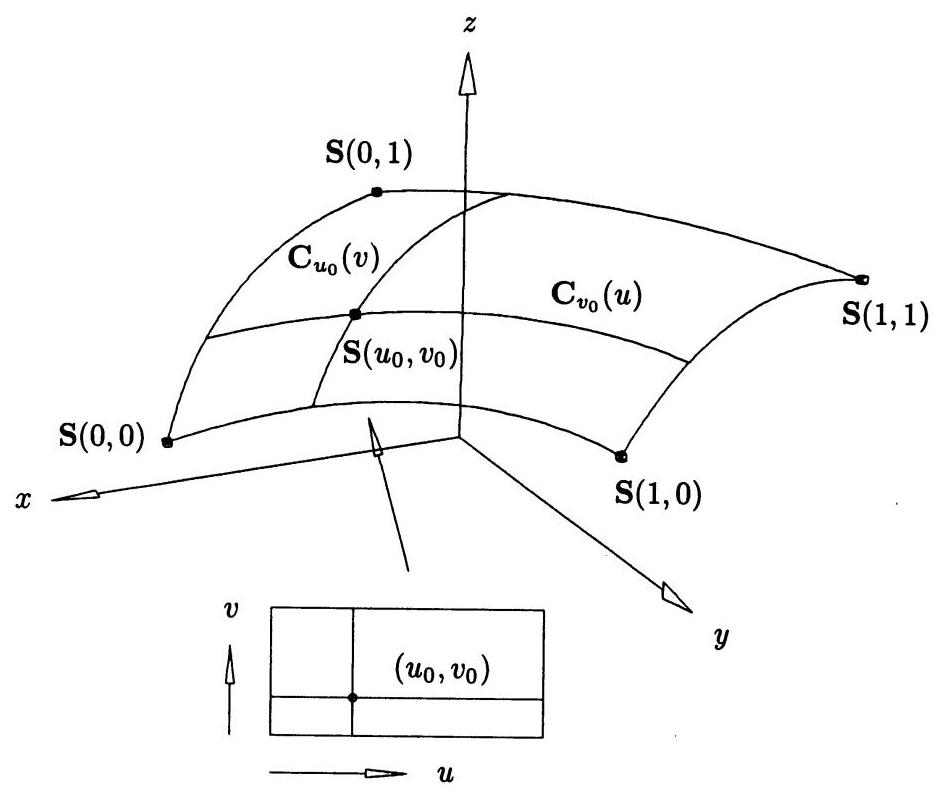
\includegraphics[max width=0.8\textwidth]{images/0193ba0d-ab19-7138-9798-cb281ce60de0_47_307_251_938_793_0.jpg}
\end{center}
\hspace*{3em} 

图 1.23. 显示等参数曲线的张量积曲面。

大括号中的项是可以通过霍纳算法 (A1.1) 评估的简单多项式，得到 \({\mathbf{b}}_{0},{\mathbf{b}}_{1},\ldots ,{\mathbf{b}}_{n}\) 。使用基数并重新应用该算法，我们获得曲面上的点。因此，我们有算法 A1.6。

\HRule

ALGORITHM A1.6

\hspace*{2em} Horner2(a, n, u0, v0, S)

\hspace*{5em} \{ /* Compute point on a power basis surface. */

\hspace*{8em} /* Input: a, n, m, u0, v0 */

\hspace*{8em} /* Output: S */

\hspace*{5em} for (i = 0; i<=n; i++)

\hspace*{7em} Horner1(a[i][], m, v0, b[i]); /* a[i][] is the ith row */

\hspace*{4em} Horner1(b, n, u0, S);

\hspace*{4em} \}

\HRule

算法 A1.6 是张量积曲面的典型算法。它们通常可以通过从曲线算法扩展而来，通常通过在一个方向上处理 \(n\) (或 \(m\) )系数的行(作为曲线)，然后在另一个方向上处理一行或多行。

对方程 (1.21) 进行求导，我们得到

\[
{\mathbf{S}}_{u}\left( {u,v}\right)  = \mathop{\sum }\limits_{{i = 1}}^{n}\mathop{\sum }\limits_{{j = 0}}^{m}i{\mathbf{a}}_{i,j}{u}^{i - 1}{v}^{j}\;{\mathbf{S}}_{v}\left( {u,v}\right)  = \mathop{\sum }\limits_{{i = 0}}^{n}\mathop{\sum }\limits_{{j = 1}}^{m}j{\mathbf{a}}_{i,j}{u}^{i}{v}^{j - 1}
\]

注意，对于固定的 \(\left( {{u}_{0},{v}_{0}}\right) ,{\mathbf{S}}_{u}\left( {{u}_{0},{v}_{0}}\right)  = {\mathbf{C}}_{{v}_{0}}^{\prime }\left( {u}_{0}\right)\) 和 \({\mathbf{S}}_{v}\left( {{u}_{0},{v}_{0}}\right)  = {\mathbf{C}}_{{u}_{0}}^{\prime }\left( {v}_{0}\right)\) 。法向量 \(\mathbf{N}\) 是使用方程 (1.4) 计算的。

非理性贝塞尔曲面是通过取控制点的双向网格和单变量伯恩斯坦多项式的乘积获得的。

\[
\mathbf{S}\left( {u,v}\right)  = \mathop{\sum }\limits_{{i = 0}}^{n}\mathop{\sum }\limits_{{j = 0}}^{m}{B}_{i,n}\left( u\right) {B}_{j,m}\left( v\right) {\mathbf{P}}_{i,j}\;0 \leq  u,v \leq  1 \tag{1.23}
\]

基函数 \({B}_{0,2}\left( u\right) {B}_{1,3}\left( v\right)\) 如图 1.24a 所示，图 1.24b 显示了一个二次 \(\times\) 三次贝塞尔曲面。

对于固定的 \(u = {u}_{0}\)

\[
{\mathbf{C}}_{{u}_{0}}\left( v\right)  = \mathbf{S}\left( {{u}_{0},v}\right)  = \mathop{\sum }\limits_{{i = 0}}^{n}\mathop{\sum }\limits_{{j = 0}}^{m}{B}_{i,n}\left( {u}_{0}\right) {B}_{j,m}\left( v\right) {\mathbf{P}}_{i,j}
\]

\[
= \mathop{\sum }\limits_{{j = 0}}^{m}{B}_{j,m}\left( v\right) \left( {\mathop{\sum }\limits_{{i = 0}}^{n}{B}_{i,n}\left( {u}_{0}\right) {\mathbf{P}}_{i,j}}\right)
\]

\[
= \mathop{\sum }\limits_{{j = 0}}^{m}{B}_{j,m}\left( v\right) {\mathbf{Q}}_{j}\left( {u}_{0}\right)  \tag{1.24}
\]

其中 \(\;{\mathbf{Q}}_{j}\left( {u}_{0}\right)  = \mathop{\sum }\limits_{{i = 0}}^{n}{B}_{i,n}\left( {u}_{0}\right) {\mathbf{P}}_{i,j}\;j = 0,\ldots ,m\)

是一个位于表面上的贝塞尔曲线。类似地， \({\mathbf{C}}_{{v}_{0}}\left( u\right)  = \mathop{\sum }\limits_{{i = 0}}^{n}{B}_{i,n}\left( u\right) {\mathbf{Q}}_{i}\left( {v}_{0}\right)\) 是一个位于表面上的贝塞尔 \(u\) 等值线。

\begin{center}
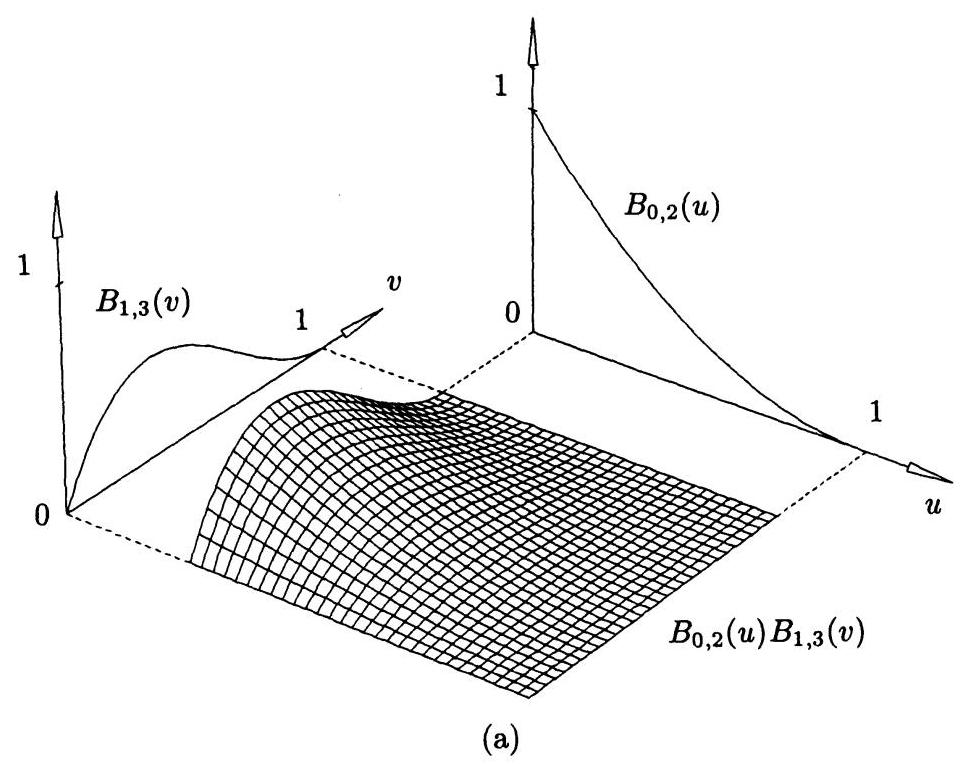
\includegraphics[max width=0.8\textwidth]{images/0193ba0d-ab19-7138-9798-cb281ce60de0_48_278_1318_960_764_0.jpg}
\end{center}
\hspace*{3em} 

图 1.24. (a) 贝塞尔张量积基函数， \({B}_{0,2}\left( u\right) {B}_{1,3}\left( v\right)\) ; (b) 二次 \(\times\) 三次贝塞尔曲面。

与曲线的情况一样，由于其优良的特性，贝塞尔曲面比幂基曲面更适合几何建模应用。特别是，

\begin{itemize}
\item 非负性: \({B}_{i,n}\left( u\right) {B}_{j,m}\left( v\right)  \geq  0\) 对所有 \(i,j,u,v\) 成立；
\end{itemize}

\begin{itemize}
\item 单位分割: \(\mathop{\sum }\limits_{{i = 0}}^{n}\mathop{\sum }\limits_{{j = 0}}^{m}{B}_{i,n}\left( u\right) {B}_{j,m}\left( v\right)  = 1\) 对所有 \(u\) 和 \(v\) 适用；
\end{itemize}

\begin{itemize}
\item \(\mathbf{S}\left( {u,v}\right)\) 包含在其控制点的凸包内；
\end{itemize}

\begin{itemize}
\item 变换不变性；
\end{itemize}

\begin{itemize}
\item 表面插值四个角控制点；
\end{itemize}

\begin{itemize}
\item 当进行三角剖分时，控制网形成表面的平面多面体近似。
\end{itemize}

有趣的是，目前尚无已知的贝塞尔曲面变差性质(见 [Prau92])。

deCasteljau 算法 (A1.5) 也可以轻松扩展以计算贝塞尔曲面上的点。参见方程 (1.24) 和图 1.25。设 \(\left( {{u}_{0},{v}_{0}}\right)\) 为固定值。对于固定的 \({j}_{0},{\mathbf{Q}}_{{j}_{0}}\left( {u}_{0}\right)  = \mathop{\sum }\limits_{{i = 0}}^{n}{B}_{i,n}\left( {u}_{0}\right) {\mathbf{P}}_{i,{j}_{0}}\) ，通过将 deCasteljau 算法应用于 \({j}_{0}\) 行的控制点，即 \(\left\{  {\mathbf{P}}_{i,{j}_{0}}\right\}  ,i = 0,\ldots ,n\) ，可以得到点。因此，将 deCasteljau 算法应用 \(\left( {m + 1}\right)\) 次得到 \({\mathbf{C}}_{{u}_{0}}\left( v\right)\) ；再将其应用一次于 \({\mathbf{C}}_{{u}_{0}}\left( v\right)\) 在 \(v = {v}_{0}\) 处得到 \({\mathbf{C}}_{{u}_{0}}\left( {v}_{0}\right)  = \mathbf{S}\left( {{u}_{0},{v}_{0}}\right)\) 。这个过程需要

\[
\frac{n\left( {n + 1}\right) \left( {m + 1}\right) }{2} + \frac{m\left( {m + 1}\right) }{2} \tag{1.25}
\]

\begin{center}
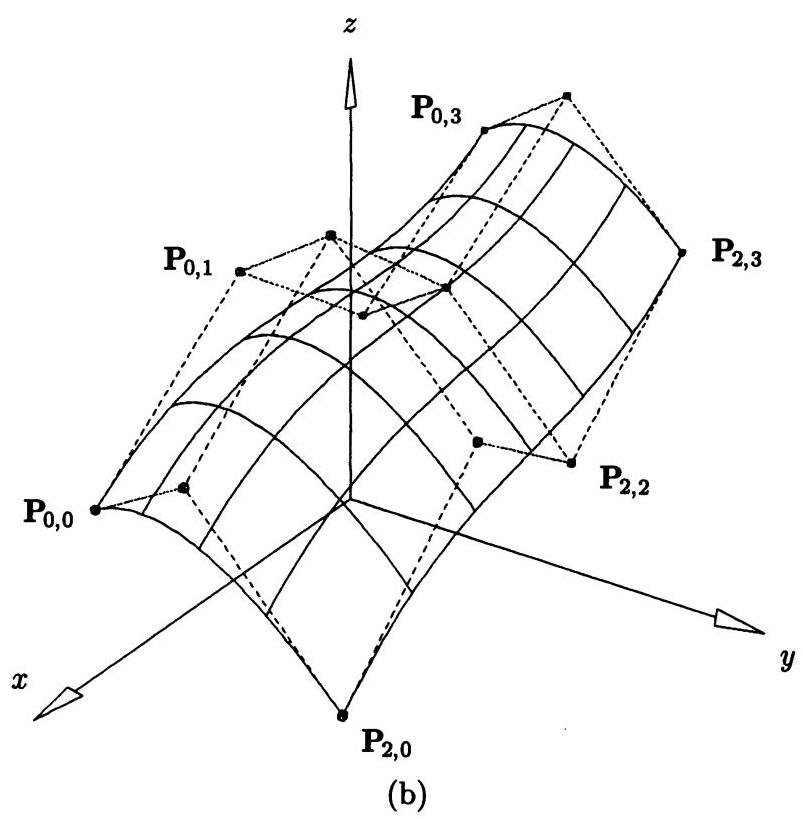
\includegraphics[max width=0.7\textwidth]{images/0193ba0d-ab19-7138-9798-cb281ce60de0_49_358_1302_803_819_0.jpg}
\end{center}
\hspace*{3em} 

图 1.24. (续)

线性插值(见练习 1.21)。通过对称性，我们可以先计算 \({\mathbf{C}}_{{v}_{0}}\left( u\right)\) ( \(n + 1\) 次 deCasteljau 应用)，然后计算 \({\mathbf{C}}_{{v}_{0}}\left( {u}_{0}\right)  = \mathbf{S}\left( {{u}_{0},{v}_{0}}\right)\) 。

这需要

\[
\frac{m\left( {m + 1}\right) \left( {n + 1}\right) }{2} + \frac{n\left( {n + 1}\right) }{2} \tag{1.26}
\]

线性插值。因此，如果 \(n > m\) 先计算 \({\mathbf{C}}_{{v}_{0}}\left( u\right)\) ，则 \({\mathbf{C}}_{{v}_{0}}\left( {u}_{0}\right)\) ；否则，先计算 \({\mathbf{C}}_{{u}_{0}}\left( v\right)\) ，然后 \({\mathbf{C}}_{{u}_{0}}\left( {v}_{0}\right)\) 。

\HRule

ALGORITHM A1.7

\hspace*{2em} deCasteljau2(P, n, m, u0, v0, S)

\hspace*{3em} \{ /* Compute a point on a Bézier surface */

\hspace*{6em} /* by the deCasteljau. */

\hspace*{6em} /* Input: P, n, m, u0, v0 */

\hspace*{6em} /* Output: S

\hspace*{3em} if (n <= m)

\hspace*{5em} \{

\hspace*{5em} for (j=0; j<=m; j++) /* P[j][] is jth row */

\hspace*{7em} deCasteljau1(P[j][], n, u0, Q[j]);

\hspace*{5em} deCasteljau1(Q, m, v0, S);

\hspace*{5em} \}

\hspace*{4em} else

\hspace*{5em} \{

\hspace*{5em} for (i = 0; i<=n; i++)

\HRule

\begin{center}
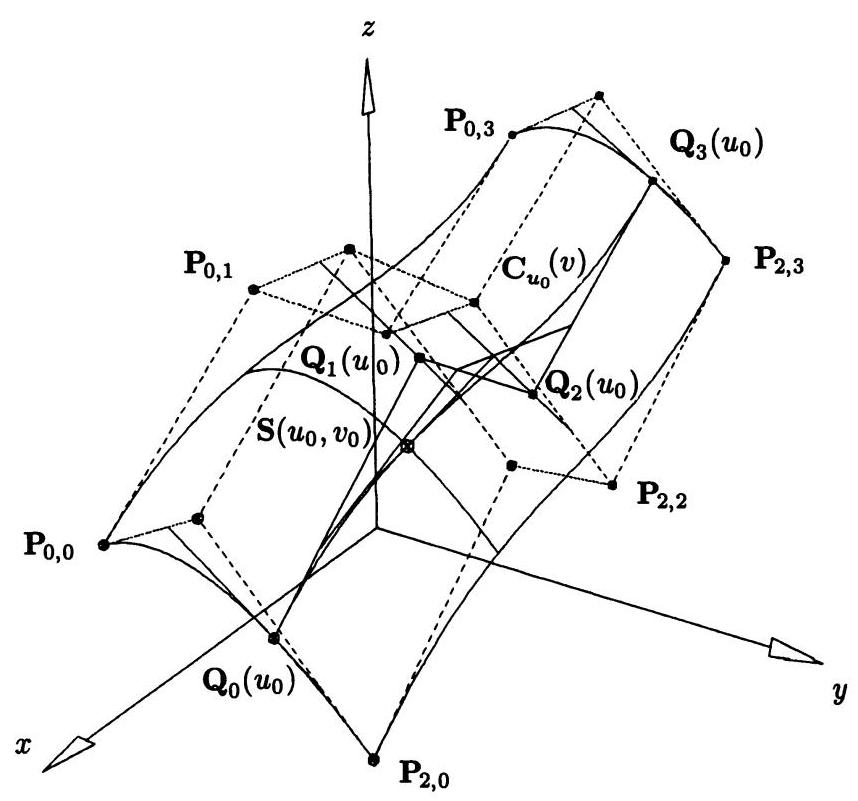
\includegraphics[max width=0.7\textwidth]{images/0193ba0d-ab19-7138-9798-cb281ce60de0_50_354_1275_858_801_0.jpg}
\end{center}
\hspace*{3em} 

图 1.25. deCasteljau 算法用于 Bézier 曲面。

\HRule

\hspace*{2em} deCasteljau1(P[][i], m, v0, Q[i]);

\hspace*{1em} deCasteljau1(Q, n, u0, S);

\hspace*{1em} \}

\}

\HRule

我们定义有理 Bézier 曲面为四维多项式 Bézier 曲面的透视投影(见 [Pieg86; Fari89])。

\[
{\mathbf{S}}^{w}\left( {u,v}\right)  = \mathop{\sum }\limits_{{i = 0}}^{n}\mathop{\sum }\limits_{{j = 0}}^{m}{B}_{i,n}\left( u\right) {B}_{j,m}\left( v\right) {\mathbf{P}}_{i,j}^{w} \tag{1.27}
\]

和

\[
\mathbf{S}\left( {u,v}\right)  = H\left\{  {{\mathbf{S}}^{w}\left( {u,v}\right) }\right\}   = \frac{\mathop{\sum }\limits_{{i = 0}}^{n}\mathop{\sum }\limits_{{j = 0}}^{m}{B}_{i,n}\left( u\right) {B}_{j,m}\left( v\right) {w}_{i,j}{\mathbf{P}}_{i,j}}{\mathop{\sum }\limits_{{i = 0}}^{n}\mathop{\sum }\limits_{{j = 0}}^{m}{B}_{i,n}\left( u\right) {B}_{j,m}\left( v\right) {w}_{i,j}}
\]

\[
= \mathop{\sum }\limits_{{i = 0}}^{n}\mathop{\sum }\limits_{{j = 0}}^{m}{R}_{i,j}\left( {u,v}\right) {\mathbf{P}}_{i,j} \tag{1.28}
\]

where

\[
{R}_{i,j}\left( {u,v}\right)  = \frac{{B}_{i,n}\left( u\right) {B}_{j,m}\left( v\right) {w}_{i,j}}{\mathop{\sum }\limits_{{r = 0}}^{n}\mathop{\sum }\limits_{{s = 0}}^{m}{B}_{r,n}\left( u\right) {B}_{s,m}\left( v\right) {w}_{r,s}}
\]

注意到 \({R}_{i,j}\left( {u,v}\right)\) 是有理函数，但它们不是其他基函数的乘积。因此， \(\mathbf{S}\left( {u,v}\right)\) 不是张量积表面，而 \({\mathbf{S}}^{w}\left( {u,v}\right)\) 是。与曲线一样，我们通常使用方程 (1.27) 并对结果进行投影。图 1.26a 显示了一个有理基函数，图 1.26b 描绘了一个二次 \(\times\) 三次有理 Bézier 表面。将这些图与图 1.24a 和 1.24b 进行比较。

假设 \({w}_{i,j} > 0\) 对所有 \(i\) 和 \(j\) 成立，之前列出的非有理 Bézier 表面的性质(以及乘积函数 \({B}_{i,n}\left( u\right) {B}_{j,m}\left( v\right)\) )自然扩展到有理 Bézier 表面。此外，如果 \({w}_{i,j} = 1\) 对所有 \(i\) 和 \(j\) 成立，则 \({R}_{i,j}\left( {u,v}\right)  = {B}_{i,n}\left( u\right) {B}_{j,m}\left( v\right)\) ，相应的表面是非有理的。

\section*{示例}

Ex1.15 让我们构造一个圆柱面片。从第 1.4 节我们知道

该

\[
{\mathbf{C}}^{w}\left( u\right)  = \mathop{\sum }\limits_{{i = 0}}^{2}{B}_{i,2}\left( u\right) {\mathbf{P}}_{i}^{w}
\]

对于 \(\left\{  {\mathbf{P}}_{i}^{w}\right\}   = \{ \left( {0,1,0,1}\right) ,\left( {0,1,1,1}\right) ,\left( {0,0,2,2}\right) \}\) ，是在 \({yz}\) 平面中的一个圆弧。使用平移(P1.14，第 1.4 节)

\[
{\mathbf{C}}_{0}^{w}\left( u\right)  = \mathop{\sum }\limits_{{i = 0}}^{2}{B}_{i,2}\left( u\right) {\mathbf{P}}_{i,0}^{w}\;\text{ and }\;{\mathbf{C}}_{1}^{w}\left( u\right)  = \mathop{\sum }\limits_{{i = 0}}^{2}{B}_{i,2}\left( u\right) {\mathbf{P}}_{i,1}^{w}
\]

\begin{center}
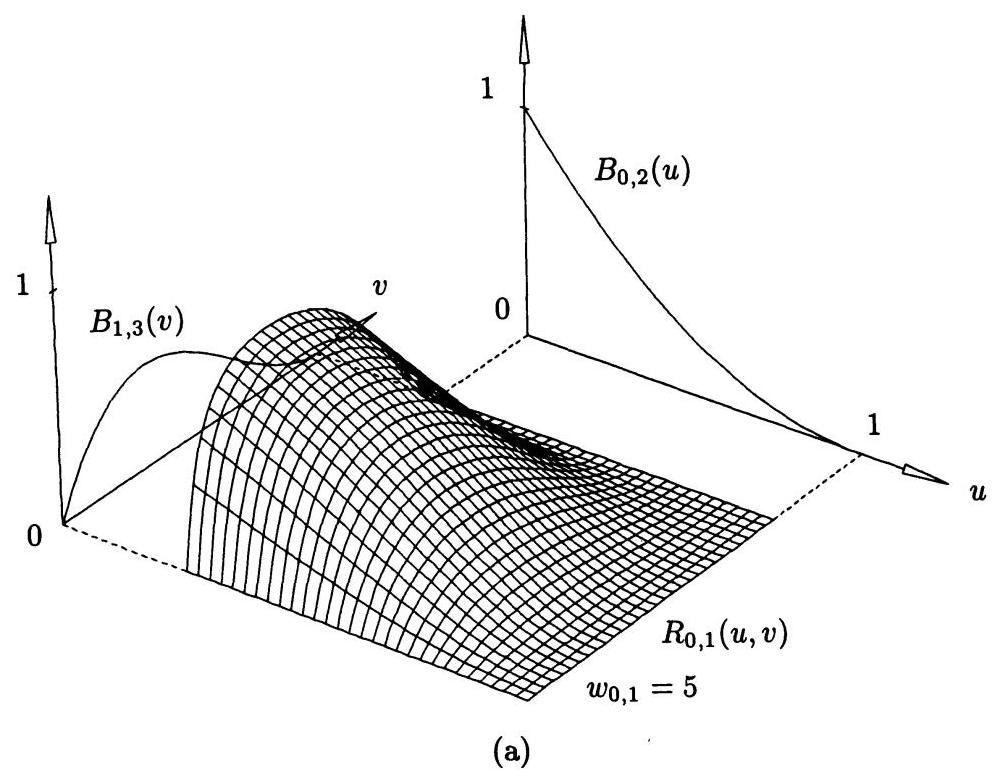
\includegraphics[max width=0.9\textwidth]{images/0193ba0d-ab19-7138-9798-cb281ce60de0_52_262_262_997_777_0.jpg}
\end{center}
\hspace*{3em} 

图 1.26. (a) 有理基函数 \({R}_{0,1}\left( {u,v}\right)\) (其中 \({w}_{0,1} = 5\) 和所有其他权重均为零)；(b) 二次 \(\times\) 三次有理 Bézier 曲面。

在哪里

\[
\left\{  {\mathbf{P}}_{i,0}^{w}\right\}   = \{ \left( {1,1,0,1}\right) ,\left( {1,1,1,1}\right) ,\left( {2,0,2,2}\right) \}
\]

和

\[
\left\{  {\mathbf{P}}_{i,1}^{w}\right\}   = \{ \left( {-1,1,0,1}\right) ,\left( {-1,1,1,1}\right) ,\left( {-2,0,2,2}\right) \}
\]

是分别位于 \(x = 1\) 和 \(x =  - 1\) 平面中的圆弧(见图 1.27)。在 \({\mathbf{C}}_{0}^{w}\) 和 \({\mathbf{C}}_{1}^{w}\) 之间进行线性插值会产生一个圆柱面，即

\[
{\mathbf{S}}^{w}\left( {u,v}\right)  = \mathop{\sum }\limits_{{i = 0}}^{2}\mathop{\sum }\limits_{{j = 0}}^{1}{B}_{i,2}\left( u\right) {B}_{j,1}\left( v\right) {\mathbf{P}}_{i,j}^{w}
\]

对于固定的 \(u = {u}_{0},{\mathbf{C}}_{{u}_{0}}^{w}\left( v\right)  = \mathop{\sum }\limits_{{j = 0}}^{1}{B}_{j,1}\left( v\right) {\mathbf{Q}}_{j}^{w}\left( {u}_{0}\right)\) ，是从 \({\mathbf{C}}_{0}^{w}\left( {u}_{0}\right)\) 到 \({\mathbf{C}}_{1}^{w}\left( {u}_{0}\right)\) 的一条平行于 \(x\) 轴的直线段。对于固定的 \(v = {v}_{0}\) ， \({\mathbf{C}}_{{v}_{0}}^{w} = {\mathbf{S}}^{w}\left( {u,{v}_{0}}\right)  = \mathop{\sum }\limits_{{i = 0}}^{2}{B}_{i,2}\left( u\right) {\mathbf{Q}}_{i}^{w}\left( {v}_{0}\right)\) 是平面 \(x = \left( {1 - {v}_{0}}\right) \left( 1\right)  + {v}_{0}\left( {-1}\right)  = 1 - 2{v}_{0}\) 中的一个圆弧。现在让我们使用算法 A1.7 计算点 \(\mathbf{S}\left( {1/2,1/2}\right)\) 。注意 \(n > m\) 。首先获得 \({\mathrm{C}}_{{v}_{0} = 1/2}^{w}\left( u\right)\)

\[
\left( {1,1,0,1}\right)
\]

\[
\left( {0,1,0,1}\right)  = {\mathbf{Q}}_{0}^{w}\left( {v}_{0}\right)
\]

(-1,1,0,1) (1,1,1,1)

(-1,1,1,1)
\[
\left( {0,1,1,1}\right)  = {\mathbf{Q}}_{1}^{w}\left( {v}_{0}\right)
\]

(2,0,2,2)

\[
\text{ (-2,0,2,2) }
\]

\[
\left( {0,0,2,2}\right)  = {\mathbf{Q}}_{2}^{w}\left( {v}_{0}\right)
\]

\begin{center}
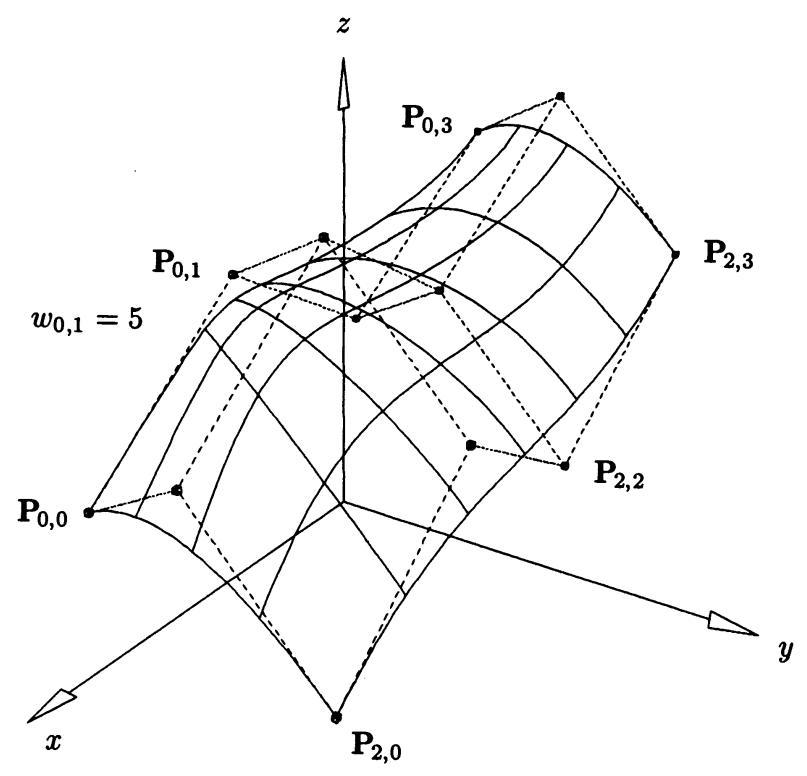
\includegraphics[max width=0.7\textwidth]{images/0193ba0d-ab19-7138-9798-cb281ce60de0_53_368_256_807_776_0.jpg}
\end{center}
\hspace*{3em} 

(b)

图 1.26. (b) (续)

现在 \({\mathbf{C}}_{{v}_{0} = 1/2}^{w}\left( u\right)  = \mathop{\sum }\limits_{{i = 0}}^{2}{B}_{i,2}\left( u\right) {\mathbf{Q}}_{i}^{w}\left( {v}_{0}\right)\) 是 \({yz}\) 平面中的圆弧

平面。然后

(0,1,0,1)

\[
\left( {0,1,\frac{1}{2},1}\right)
\]

\[
\left( {0,\frac{3}{4},1,\frac{5}{4}}\right)  = {\mathbf{S}}^{w}\left( {\frac{1}{2},\frac{1}{2}}\right)
\]

\[
\left( {0,\frac{1}{2},\frac{3}{2},\frac{3}{2}}\right)
\]

\[
\left( {0,0,2,2}\right)
\]

投影得到

\[
\mathbf{S}\left( {\frac{1}{2},\frac{1}{2}}\right)  = H\left\{  \left( {0,\frac{3}{4},1,\frac{5}{4}}\right) \right\}   = \left( {0,\frac{3}{5},\frac{4}{5}}\right)
\]

练习 43

\begin{center}
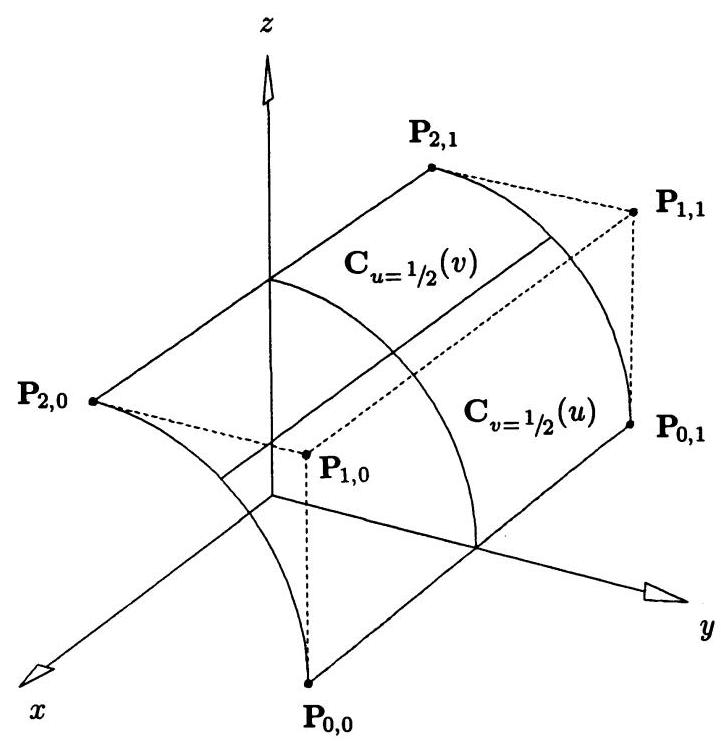
\includegraphics[max width=0.6\textwidth]{images/0193ba0d-ab19-7138-9798-cb281ce60de0_54_391_268_725_744_0.jpg}
\end{center}
\hspace*{3em} 

图 1.27. 作为有理 Bézier 曲面的圆柱面片。

\section*{练习}

1.1. 考虑由方程 (1.1) 和 (1.2) 给出的圆弧的两个参数表示。使用方程 (1.1) 计算曲线在 \(u = \pi /4\) 的点，并使用方程 (1.2) 计算在 \(t = 1/2\) 的点。解释结果。

1.2. 计算方程 (1.1) 的加速度向量 \({\mathbf{C}}^{\prime \prime }\left( u\right)\) 。解释结果。

1.3. 使用三角函数，给出有界表面的参数定义

\begin{itemize}
\item 一个以原点为顶点，轴对称沿 \(z\) 轴的直圆锥；
\end{itemize}

\begin{itemize}
\item 该圆锥向上打开，并在 \(z = 2\) 处被半径为 \(= 1\) 的圆界定。
\end{itemize}

修改方程 (1.2) 以获得同一圆锥的另一表示。计算三角表示的第一个偏导数 \({\mathbf{S}}_{u}\) 和 \({\mathbf{S}}_{v}\) 。这些导数在圆锥顶点处的值是多少？

1.4. 考虑抛物线弧 \(\mathbf{C}\left( u\right)  = \left( {x\left( u\right) ,y\left( u\right) }\right)  = \left( {-1 - u + 2{u}^{2}, - {2u} + {u}^{2}}\right)\) ， \(0 < u < 1\) 。绘制此曲线。通过对函数 \(x\left( u\right)\) 和 \(y\left( u\right)\) 应用变换来旋转和平移该曲线。应用这两个变换

(1) \({90}^{ \circ  }\) 关于原点的旋转。旋转矩阵(从左侧应用)为

\[
\left\lbrack  \begin{array}{rr} 0 &  - 1 \\  1 & 0 \end{array}\right\rbrack
\]

(2) 使用向量 (-1, -1) 进行平移。

底层抛物线的隐式方程为 \({x}^{2} - {4xy} + 4{y}^{2} - {4x} - y - 5 = 0\) 。绘制此曲线。将先前的旋转和平移应用于此方程。提示:让 \(\bar{x},\bar{y}\) 为变换后的坐标。找到表达式 \(x = f\left( {\bar{x},\bar{y}}\right)\) 和 \(y = g\left( {\bar{x},\bar{y}}\right)\) ，并将这些代入隐式方程以获得变换后抛物线的隐式方程。

1.5. 确定计算一个 \(n\) 次三维幂基曲线上的点所需的加法和乘法的公式。

1.6. 构造一个带有环的三次幂基曲线。提示:考虑需要什么样的端点和端导数， \({\mathbf{C}}^{\prime }\left( 0\right)\) 和 \({\mathbf{C}}^{\prime }\left( 1\right)\) 。

1.7. 构造一个带有尖点的三次幂基曲线。提示:考虑 \({\mathbf{C}}^{\prime }\left( u\right)\) 和 \({\mathbf{C}}^{\prime \prime }\left( u\right)\) 。草图展示 \({x}^{\prime }\left( u\right) ,{y}^{\prime }\left( u\right) ,{x}^{\prime \prime }\left( u\right)\) 和 \({y}^{\prime \prime }\left( u\right)\) 作为 \(u\) 的函数应呈现的样子。确定一个合适的 \({\mathbf{C}}^{\prime \prime }\left( u\right)\) ，然后进行积分以获得 \({\mathbf{C}}^{\prime }\left( u\right)\) 和 \(\mathbf{C}\left( u\right)\) 。

1.8. 构造一个带有拐点的三次幂基曲线。

1.9. 设 \(\mathbf{C}\left( u\right)  = \left( {x\left( u\right) ,y\left( u\right) }\right)  = \left( {1 + u - 2{u}^{2} + {u}^{3},1 - {2u} + {u}^{3}}\right) , - 1 \leq  u \leq  1\) 。设 \(u = {2v} - 1\) 。通过在 \(\mathbf{C}\left( u\right)\) 中将 \({2v} - 1\) 替换为 \(u\) 来推导曲线 \(\mathbf{C}\left( v\right)\) 。曲线 \(\mathbf{C}\left( v\right)\) 的度数是多少？计算 \(\mathbf{C}\left( u\right)\) 对于 \(u =  - 1,0,1\) 。计算 \(\mathbf{C}\left( v\right)\) 对于 \(v = 0,1/2,1\) 。你对曲线 \(\mathbf{C}\left( u\right)\) 和 \(\mathbf{C}\left( v\right)\) 有什么看法？ \(\mathbf{C}\left( v\right)\) 被称为 \(\mathbf{C}\left( u\right)\) 的重新参数化。

1.10. 检查伯恩斯坦多项式在 \(n = 2\) 和 \(n = 3\) 情况下的性质 P1.7。

1.11. 有时需要反转一条曲线，即，给定 \({\mathbf{C}}_{1}\left( u\right) ,0 \leq  u \leq  1\) ，生成 \({\mathbf{C}}_{2}\left( v\right) ,0 \leq  v \leq  1\) ，使得这两条曲线在几何上是相同的，但 \({\mathbf{C}}_{1}\left( 0\right)  = {\mathbf{C}}_{2}\left( 1\right)\) 和 \({\mathbf{C}}_{1}\left( 1\right)  = {\mathbf{C}}_{2}\left( 0\right)\) 不同。你将如何使用贝塞尔形式来实现这一点？使用幂基形式呢？

1.12. 考虑由控制点 \({\mathbf{P}}_{0} = \left( {0,6}\right)\) , \({\mathbf{P}}_{1} = \left( {3,6}\right) ,{\mathbf{P}}_{2} = \left( {6,3}\right) ,{\mathbf{P}}_{3} = \left( {6,0}\right)\) 给出的 \({xy}\) 平面三次 Bézier 曲线。使用 deCasteljau 算法计算点 \(\mathbf{C}\left( {1/3}\right)\) 。直接使用公式 (1.7) 和 (1.8) 计算相同的点，即在 \(u = 1/3\) 处评估基函数并乘以相应的控制点。

1.13. 确定使用 de Casteljau 算法、A1.5 和算法 A1.4 计算 \(n\) 阶三维 Bézier 曲线上的一个点所需的加法和乘法的公式。将结果与练习 1.5(霍纳算法)进行比较。

1.14. 对于给定的 \(n\) ，行向量 \(\left\lbrack  {{B}_{0,n}\left( u\right) ,\ldots ,{B}_{n,n}\left( u\right) }\right\rbrack\) 可以写成 \(\left\lbrack  {1,u,\ldots ,{u}^{n}}\right\rbrack  M\) ，其中 \(M\) 是一个 \(\left( {n + 1}\right)  \times  \left( {n + 1}\right)\) 矩阵。因此，Bézier 曲线可以用矩阵形式表示为 \(\mathbf{C}\left( u\right)  = {\left\lbrack  {u}^{i}\right\rbrack  }^{T}M\left\lbrack  {\mathbf{P}}_{i}\right\rbrack\) 。计算矩阵 \(M\) 对于 \(n = 1,2,3\) 。注意，设置 \(\left\lbrack  {\mathbf{a}}_{i}\right\rbrack   = M\left\lbrack  {\mathbf{P}}_{i}\right\rbrack\) 会将 Bézier 曲线转换为幂基形式。假设 \(0 \leq  u \leq  1,\left\lbrack  {\mathbf{P}}_{i}\right\rbrack   = {M}^{-1}\left\lbrack  {\mathbf{a}}_{i}\right\rbrack\) 给出了从幂基到 Bézier 形式的转换。

1.15. 将此与练习 1.9 进行比较。也可以在参数区间 \(\left\lbrack  {0,1}\right\rbrack\) 之外定义 Bézier 曲线。这相当于对 Bézier 曲线进行重新参数化。

曲线。设

\[
\mathbf{C}\left( u\right)  = \mathop{\sum }\limits_{{i = 0}}^{n}{B}_{i,n}\left( u\right) {\mathbf{P}}_{i}\;u \in  \left\lbrack  {0,1}\right\rbrack
\]

设定 \(v \in  \left\lbrack  {a,b}\right\rbrack\) 。然后 \(u = \left( {v - a}\right) /\left( {b - a}\right)\) 。将这个方程代入方程 (1.8) 中，并推导出重新参数化曲线的表达式

\[
\mathbf{C}\left( v\right)  = \frac{1}{{\left( b - a\right) }^{n}}\mathop{\sum }\limits_{{i = 0}}^{n}\frac{n!}{i!\left( {n - i}\right) !}{\left( v - a\right) }^{i}{\left( b - v\right) }^{n - i}{\mathbf{P}}_{i}
\]

有趣的是，控制点并没有改变，只有基函数发生了变化。幂基形式的重新参数化改变了几何系数，但没有改变基函数。

1.16. 考虑圆形

\[
\mathbf{C}\left( u\right)  = \left( {\frac{1 - {u}^{2}}{1 + {u}^{2}},\frac{2u}{1 + {u}^{2}}}\right)
\]

确定参数 \(u\) 的哪些范围产生圆的哪些象限。这些方程是否产生整个圆？你对参数化有什么看法？

1.17. 考虑以下在 \({xy}\) 平面上的有理三次 Bézier 曲线: \({\mathbf{P}}_{0} = \left( {0,6}\right)\) , \({\mathbf{P}}_{1} = \left( {3,6}\right) ,{\mathbf{P}}_{2} = \left( {6,3}\right) ,{\mathbf{P}}_{3} = \left( {6,0}\right) ,{w}_{0} = 4,{w}_{1} = 1,{w}_{2} = 1,{w}_{3} = 4\) 。通过扩展 de Casteljau 表计算点 \(\mathbf{C}\left( {2/3}\right)\) 。

1.18. 我们使用的有理函数有什么特征使我们能够使用齐次坐标表示？这种表示有什么优势？

1.19. 找到第二象限中圆弧的有理 Bézier 表示，即确定 \({\mathbf{P}}_{i}\) 和 \({w}_{i}\) 。提示:使用对称性，并通过显示 \({\left( x\left( u\right) \right) }^{2} + {\left( y\left( u\right) \right) }^{2} = 1\) 对所有 \(u \in  \left\lbrack  {0,1}\right\rbrack\) 进行检查来验证你的结果。

1.20. 第一象限中的圆弧也由以下方程给出

\[
\mathbf{C}\left( u\right)  = \left( {\frac{1 + \left( {\sqrt{2} - 2}\right) u + \left( {1 - \sqrt{2}}\right) {u}^{2}}{1 + \left( {\sqrt{2} - 2}\right) u + \left( {2 - \sqrt{2}}\right) {u}^{2}},\frac{\frac{\sqrt{2}}{2}u\left( {\left( {\sqrt{2} - 2}\right) u + 2}\right) }{1 + \left( {\sqrt{2} - 2}\right) u + \left( {2 - \sqrt{2}}\right) {u}^{2}}}\right)
\]

确定与这些方程相对应的有理 Bézier 表示。提示: \({\mathbf{P}}_{i}\) 必须与之前的 \(- \left( {1,0}\right) ,\left( {1,1}\right) ,\left( {0,1}\right)\) 相同；为什么？通过使多项式相等并替换 \(u = 0,1/2,1\) 来计算权重 \({w}_{i}\) ，如之前所做。使用任何方法计算点 \(\mathbf{C}\left( {1/2}\right)\) 。 \(\mathbf{C}\left( {1/2}\right)\) 有什么有趣之处？

1.21. 推导方程 (1.25) 和 (1.26)。提示:使用公式 \(1 + 2 + \cdots  + n = {}^{n\left( {n + 1}\right) }/2\) 。

1.22. 对于圆柱面示例 (Ex1.15)，计算等曲线 \({\mathbf{C}}_{{u}_{0} = 1/3}^{w}\left( v\right)\) 的控制点 \({\mathbf{Q}}_{j}^{w}\left( {u}_{0}\right)\) 。

1.23. 设 \(n = 3\) 和 \(m = 2\) 。考虑由控制网定义的非有理 Bézier 曲面

控制网

\[
\left\{  {\mathbf{P}}_{i,0}\right\}   = \{ \left( {0,0,0}\right) ,\left( {3,0,3}\right) ,\left( {6,0,3}\right) ,\left( {9,0,0}\right) \}
\]

\[
\left\{  {\mathbf{P}}_{i,1}\right\}   = \{ \left( {0,2,2}\right) ,\left( {3,2,5}\right) ,\left( {6,2,5}\right) ,\left( {9,2,2}\right) \}
\]

\[
\left\{  {\mathbf{P}}_{i,2}\right\}   = \{ \left( {0,4,0}\right) ,\left( {3,4,3}\right) ,\left( {6,4,3}\right) ,\left( {9,4,0}\right) \}
\]

a. 草绘该曲面；

b. 使用 deCasteljau 算法计算表面点 \(\mathbf{S}\left( {1/3,1/2}\right)\) ；

c. 固定 \({u}_{0} = 1/2\) 并提取曲线 \({\mathbf{C}}_{{u}_{0} = 1/2}\left( v\right)\) 的贝塞尔表示(控制点)。

1.24. 设

\[
\mathbf{S}\left( {u,v}\right)  = \mathop{\sum }\limits_{{i = 0}}^{n}\mathop{\sum }\limits_{{j = 0}}^{m}{B}_{i,n}\left( u\right) {B}_{j,m}\left( v\right) {\mathbf{P}}_{i,j}
\]

并假设 \({\mathbf{P}}_{0,0} = {\mathbf{P}}_{1,0} = \cdots  = {\mathbf{P}}_{n,0}\) 。这如何影响 \(\mathbf{S}\left( {u,v}\right)\) 、导数 \({\mathbf{S}}_{u}\left( {u,v}\right)\) 和 \({\mathbf{S}}_{v}\left( {u,v}\right)\) 以及曲线 \({\mathbf{C}}_{{v}_{0}}\left( u\right)\) ？假设 \({\mathbf{P}}_{i,0} = \left( {1,0,0}\right)\) 对于示例 Ex1.15，其中 \({w}_{0,0} = 1,{w}_{1,0} = 1\) 和 \({w}_{2,0} = 2\) 。你得到什么类型的表面？

1.25. 这个问题的前提是练习 1.14。 有理贝塞尔曲面(方程 [1.27])具有矩阵形式

\[
{\mathbf{S}}^{w}\left( {u,v}\right)  = {\left\lbrack  {B}_{i,n}\left( u\right) \right\rbrack  }^{T}\left\lbrack  {\mathbf{P}}_{i,j}^{w}\right\rbrack  \left\lbrack  {{B}_{j,m}\left( v\right) }\right\rbrack   = {\left\lbrack  {u}^{i}\right\rbrack  }^{T}{M}_{n}\left\lbrack  {\mathbf{P}}_{i,j}^{w}\right\rbrack  {M}_{m}^{T}\left\lbrack  {v}^{j}\right\rbrack
\]

其中 \({\left\lbrack  {u}^{i}\right\rbrack  }^{T}\) 和 \(\left\lbrack  {v}^{j}\right\rbrack\) 是向量， \({M}_{n}\) 是一个 \(\left( {n + 1}\right)  \times  \left( {n + 1}\right)\) 矩阵， \({M}_{m}^{T}\) 是一个 \(\left( {m + 1}\right)  \times\)  \(\left( {m + 1}\right)\) 矩阵，而 \(\left\lbrack  {\mathbf{P}}_{i,j}^{w}\right\rbrack\) 是一个四维点的 \(\left( {n + 1}\right)  \times  \left( {m + 1}\right)\) 矩阵。将这个形式明确写出用于圆柱面示例 Ex1.15。使用这个矩阵形式，计算点 \({\mathbf{S}}^{w}\left( {1/2,1/2}\right)\) ，然后投影以获得 \(\mathbf{S}\left( {1/2,1/2}\right)\) 。对于 \(\mathbf{S}\left( {u,v}\right)\) 没有直接的矩阵形式；为什么？


\clearpage
\end{document}
